\chapter{Results}
\label{ch:results}

\blockquote{This chapter reports the results of applying the procedures described in \hyperref[ch:methods]{Chapter 3: Data \& Methods}. I begin by demonstrating for the reader how to interpret the ternary plots used to visually represent the degree of lexical flexibility for individual items (\ref{R1}) (\secref*{sec:4.2}). Next I look at the flexibility of lexical items in English and Nuuchahnulth, both independently and in comparison (\secref*{sec:4.3}). I then I investigate whether lexical flexibility depends on corpus size (\ref{R2}) (\secref*{sec:4.4}), followed by the relationship between the degree of lexical flexibility and frequency / dispersion (\ref{R3}) (\secref*{sec:4.5}). Finally, I discuss the behavior of flexible items with respect to their semantics (\ref{R4}) (\secref*{sec:4.6}).}

\section{Introduction}
\label{sec:4.1}

This chapter presents the empirical findings of this study, answering the research questions posed in \chref{ch:introduction}. I employ a useful visualization for displaying information about lexical flexibility called a \dfn{ternary plot} or \dfn{triangle plot}; I explain how these ternary plots are to be read in \secref*{sec:4.2}. \secref*{sec:4.3} focuses on answering \ref{R1}, \enquote{How flexible are lexical items in English and Nuuchahnulth?}, both individually and in comparison. \secref*{sec:4.4} is dedicated to answering \ref{R2}, \enquote{Is there a correlation between degree of lexical flexibility and size of the corpus?}, and \secref*{sec:4.5} answers \ref{R3}, \enquote{Is there a correlation between degree of lexical flexibility for a lexical item and frequency (or corpus dispersion)?}. In the final section (\secref{sec:4.6}), I look at the semantic behavior of more and less flexible items (question \ref{R4}).

\section{Interpreting the results}
\label{sec:4.2}

In \secref*{sec:3.4.1} I describe the procedure for quantifying the lexical flexibility of an item in a corpus using a Shannon diversity index ($H$). While the resulting values nicely align with our intuitions about when a lexical item is more or less flexible, some information is lost in the process. Reducing the lexical flexibility of an item to a single number obscures the fact that items can be equally flexible in different ways. Consider the fictional frequency data for two different stems in \tabref{tab:equal-flexibility-stems}. Stem A displays a great deal of reference-predicate flexibility, but no instances of use as a modifier. Stem B, in contrast, displays extensive reference-modifier flexibility, but no instances of use as a predicate. However, the overall flexibility ratings of the two stems are the same.

\begin{table}[h!]
  \centering
  \caption{Stems with different distributions of discourse functions and the same flexibility}
  \label{tab:equal-flexibility-stems}
  \begin{tabular}{ l c c c c }
    \toprule
    stem   & reference & predication & modification & flexibility\\
    \midrule
    Stem A & 25        & 25          & 0            & 0.631      \\
    Stem B & 25        & 0           & 25           & 0.631      \\
    \bottomrule
  \end{tabular}
\end{table}

One way to address this reduction in fidelity is to report frequencies and corpus dispersions for each function in addition to the overall flexibility rating for each stem. I provide this information in \appref{app:100-item-samples} alongside each item's flexibility rating. However, it is also possible to visualize the relative usage of an item for each discourse function in an intuitive way by using a \dfn{ternary plot} (also called a \dfn{triangle plot}, \dfn{simplex plot}, \dfn{Gibbs triangle}, or \dfn{de Finetti diagram}). A ternary plot depicts the ratios of three variables as points within an equilateral triangle. Each corner of the triangle corresponds to one of the three possible categories (in this case, reference, predication, or modification). The closer a data point is to a particular corner, the larger the ratio of that category is. To illustrate with an example: \figref{fig:Eng-difficult} is a ternary plot for the functions of the word \txn{difficult} in \idx{English}, along with the underlying frequency data and resulting flexibility rating. Because the word \txn{difficult} only appears as a modifier in the corpus, it has a flexibility rating of $0$. In the ternary plot, this is evident from the fact that the plot point for \txn{difficult} sits in the modification corner of the triangle.

\begin{figure}

  \centering
  \caption{Flexibility of \idx{English} \textit{difficult}}
  \label{fig:Eng-difficult}

  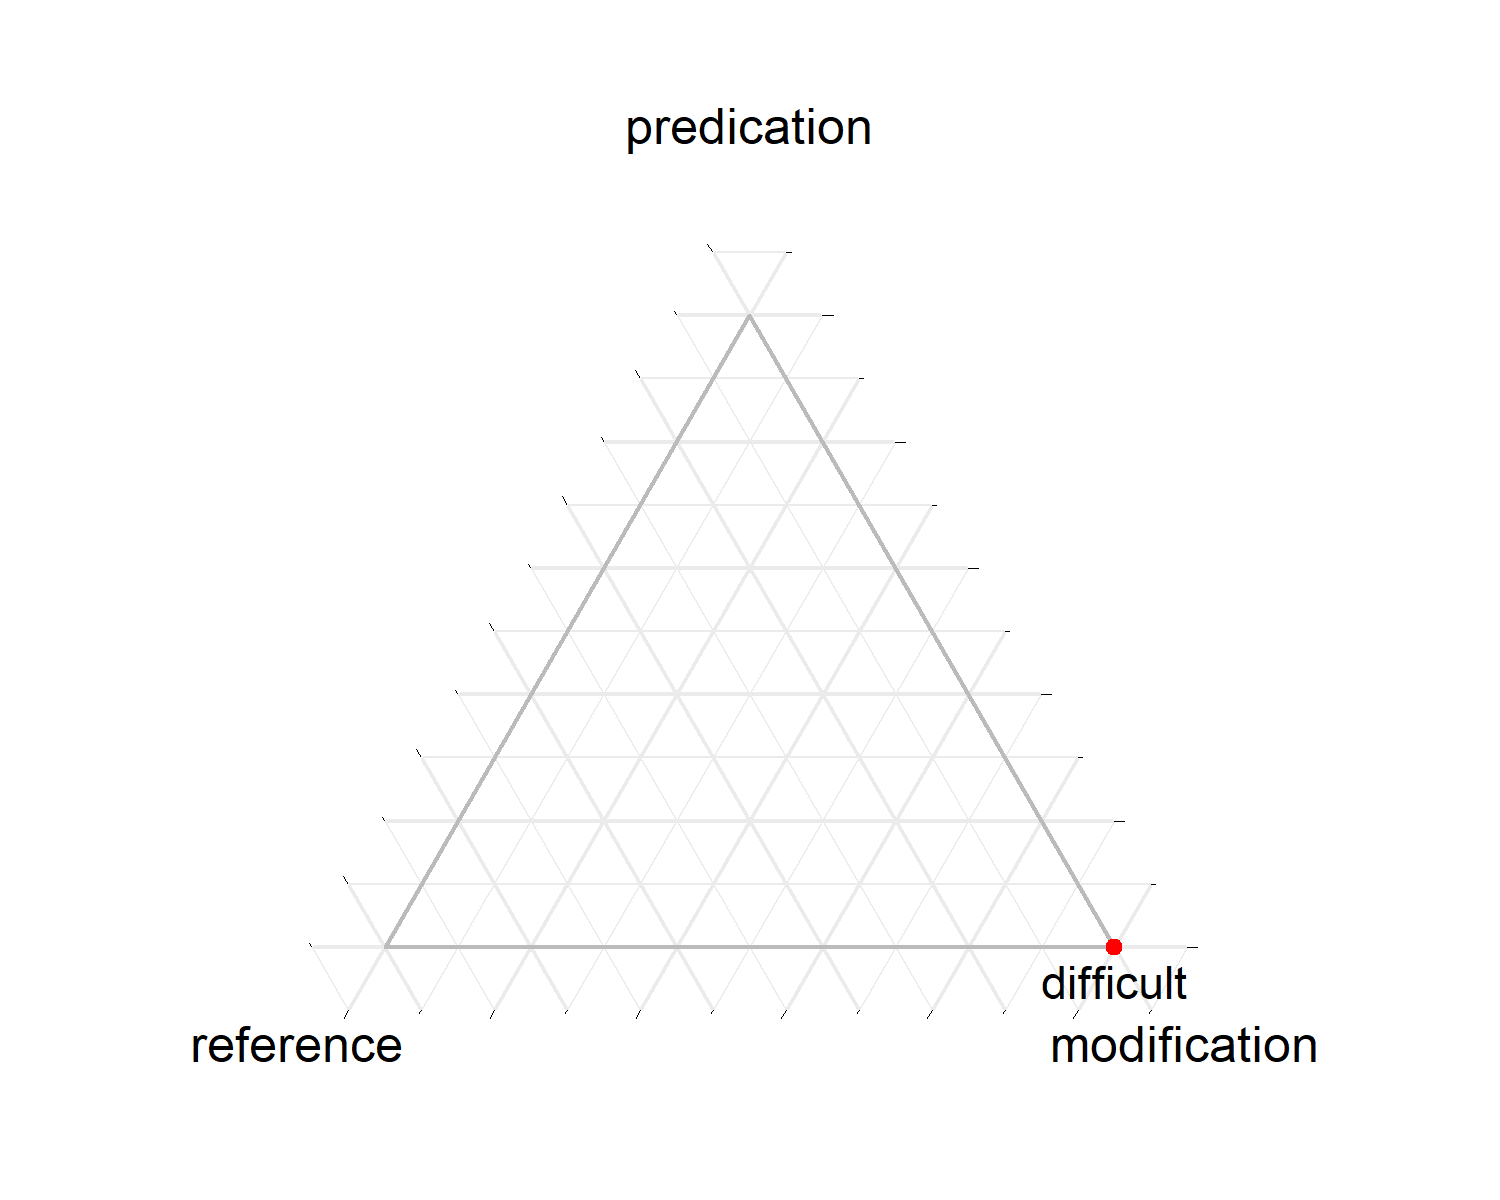
\includegraphics{Eng-difficult.png}

  \begin{tabular}{ c c c c }
    \toprule
    reference & predication & modification & flexibility\\
    \midrule
    0         & 0           & 54           & 0.000      \\
    \bottomrule
  \end{tabular}

\end{figure}

Compare the plot for \txn{difficult} in \figref{fig:Eng-difficult} to that of \txn{anything} in \figref{fig:Eng-anything}. The stem \txn{anything} also has a flexibility rating of $0$ because all of its tokens are used for reference. Even though its flexibility rating is the same as that of \txn{difficult}, it is plotted in a different corner of the ternary plot (reference).

\begin{figure}

  \centering
  \caption{Flexibility of \idx{English} \textit{anything}}
  \label{fig:Eng-anything}

  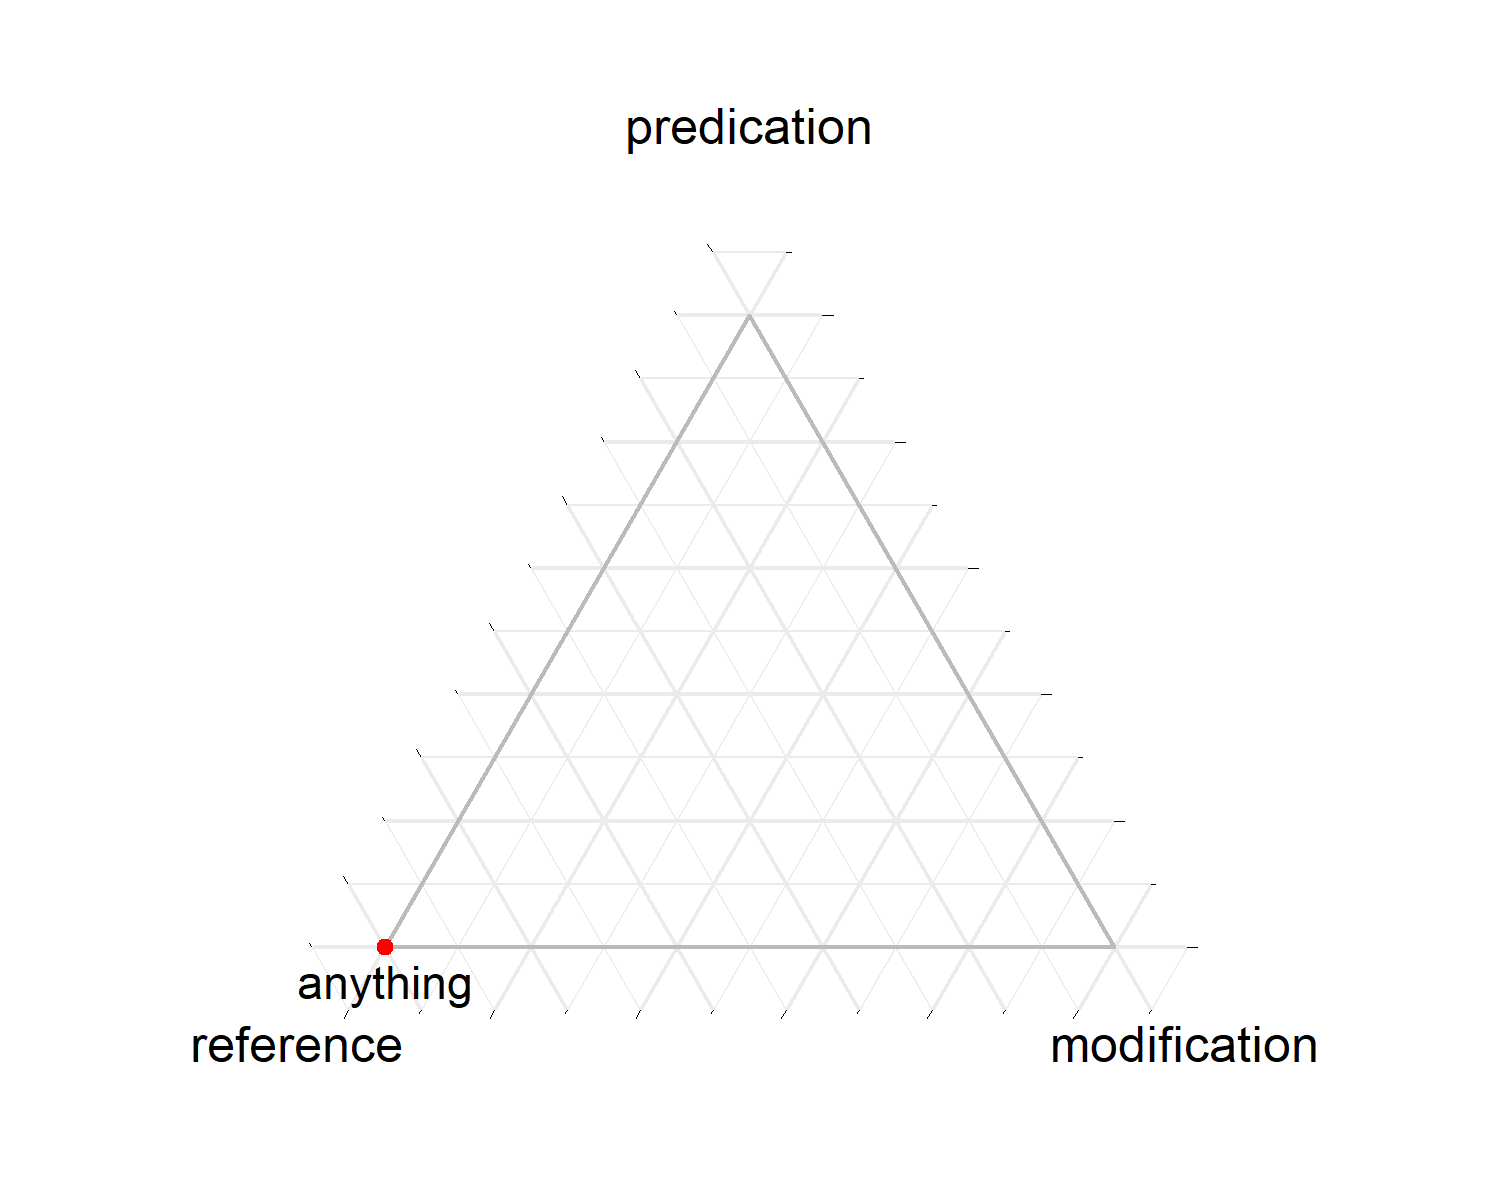
\includegraphics{Eng-anything.png}

  \begin{tabular}{ c c c c }
    \toprule
    reference & predication & modification & flexibility\\
    \midrule
    2,081     & 0           & 0            & 0.000      \\
    \bottomrule
  \end{tabular}

\end{figure}

\figref{fig:Eng-childhood} shows a case where a stem (\txn{childhood}) is flexible between reference and modification, but not predication. Finally, a perfectly flexible item which has equal use as a referent, predicate, and modifier, would sit exactly in the center of the triangle. The \idx{Nuuchahnulth} stem \txn{ʔu·q} \tln{good} is one such case, shown in \figref{fig:Nuu-good}. The closer a point is towards the center of the triangle, the more flexible it is.

\begin{figure}

  \centering
  \caption{Flexibility of \idx{English} \textit{childhood}}
  \label{fig:Eng-childhood}

  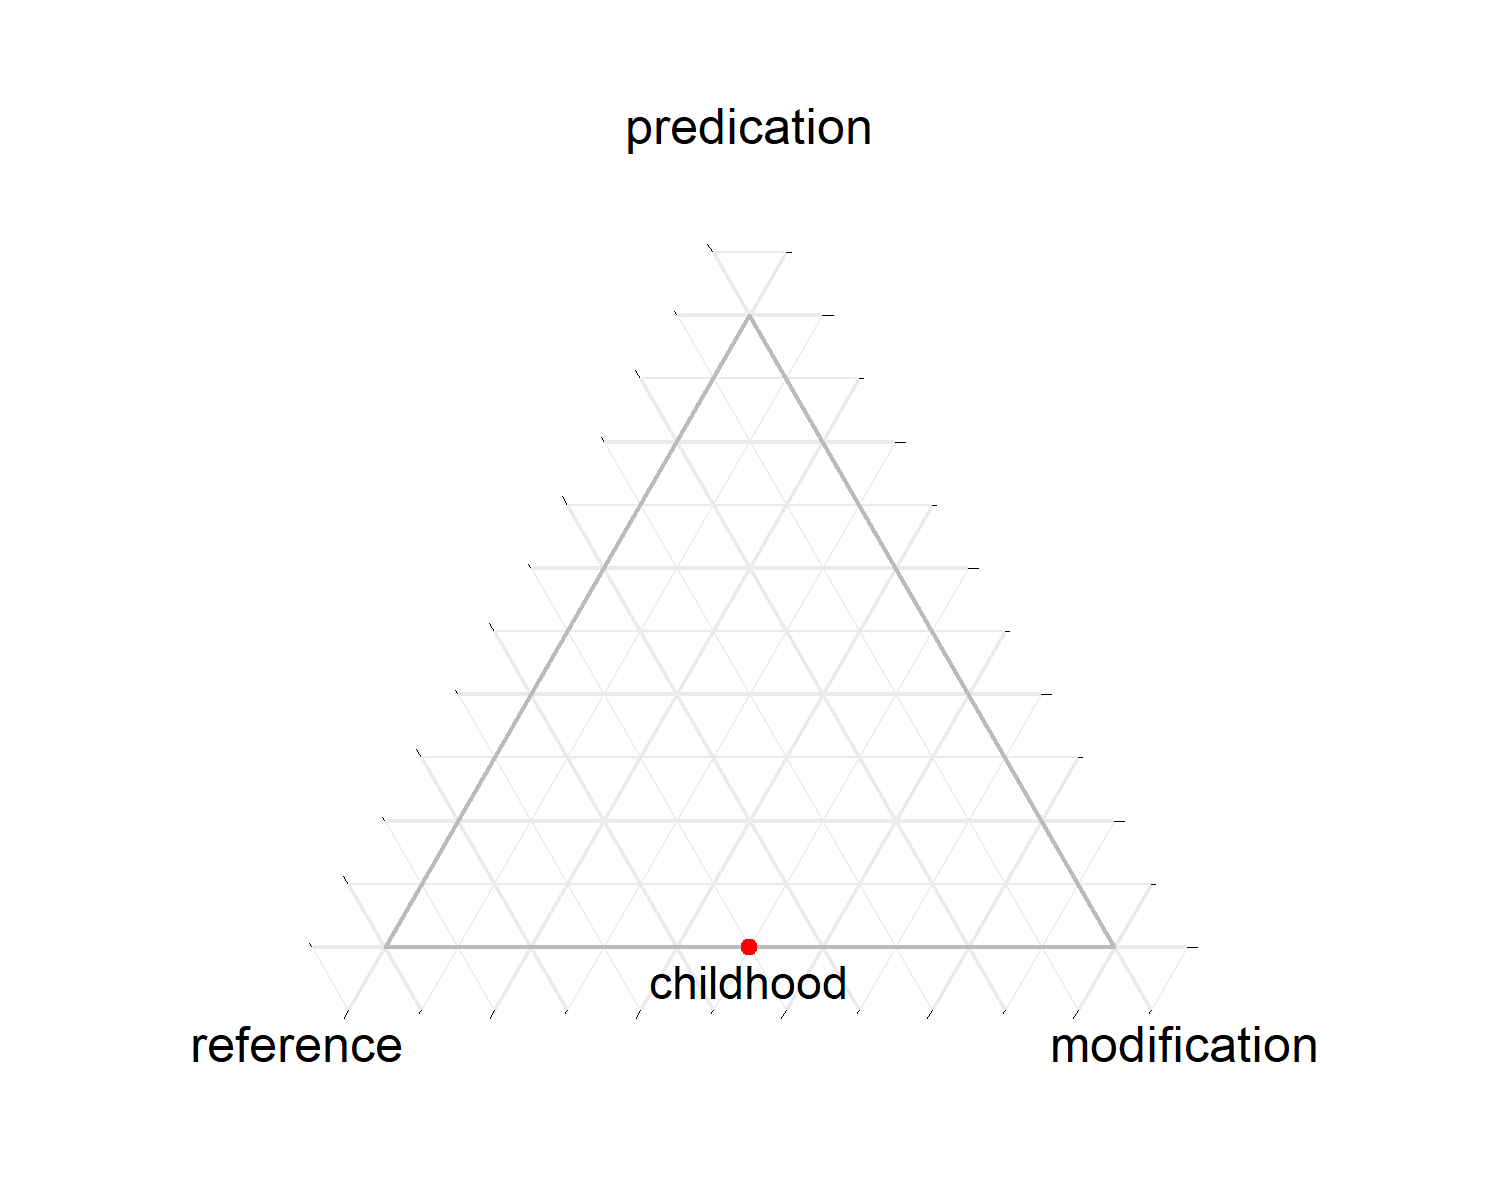
\includegraphics{Eng-childhood.png}

  \begin{tabular}{ c c c c }
    \toprule
    reference & predication & modification & flexibility\\
    \midrule
    2         & 0           & 2            & 0.631      \\
    \bottomrule
  \end{tabular}

\end{figure}

\begin{figure}

  \centering
  \caption{Flexibility of \idx{Nuuchahnulth} \textit{ʔu·q} \tln{good}}
  \label{fig:Nuu-good}

  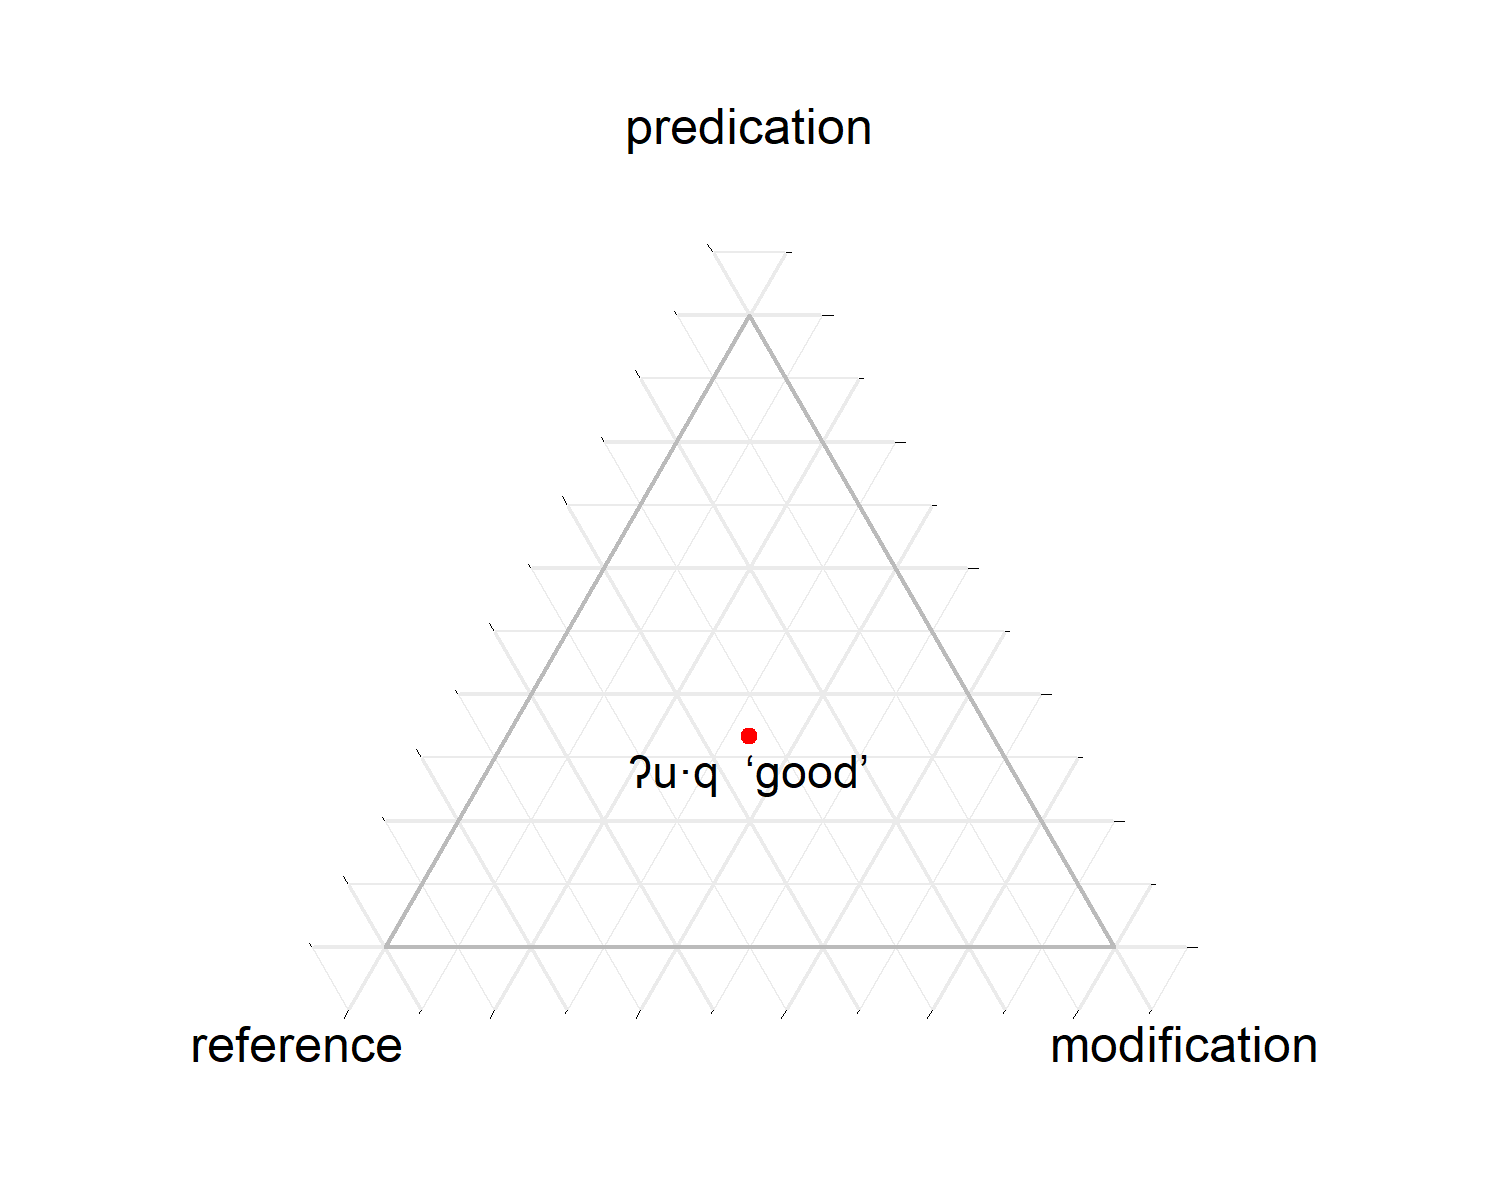
\includegraphics{Nuu-good.png}

  \begin{tabular}{ c c c c }
    \toprule
    reference & predication & modification & flexibility\\
    \midrule
    1         & 1           & 1            & 1.000      \\
    \bottomrule
  \end{tabular}

\end{figure}

Also remember from \chref{ch:methods} that corpus dispersion is a better measure of frequency of exposure than just raw frequency. Thus in addition to relative frequency data, I also report corpus dispersions for the discourse functions of each lexical item in \appref{app:100-item-samples}. Note that the corpus dispersions are calculated separately for each discourse function (in addition to the overall corpus dispersion of the lexical item). A particular lexical item might be used for one function evenly throughout the corpus, and thus have a low $DP$ for that function, but might only be used for another function in one or two texts, thus giving that function a high $DP$. The ratios of these corpus dispersions for each function can be plotted on a ternary plot just like frequency. Plots based on corpus dispersions are sometimes notably different from plots based on frequencies, as \figref{fig:plot-frequency-vs-dispersion} illustrates for the English word \txn{favorite}. In most cases however the plots are identical or near-identical. As such, for the remainder of this study I will use ternary plots based on corpus dispersion rather than frequency, noting where the two diverge only when relevant.

\begin{landscape}
\begin{figure}

  \centering
  \caption{Flexibility using frequency vs. corpus dispersion for \idx{English} \textit{favorite}}
  \label{fig:plot-frequency-vs-dispersion}

  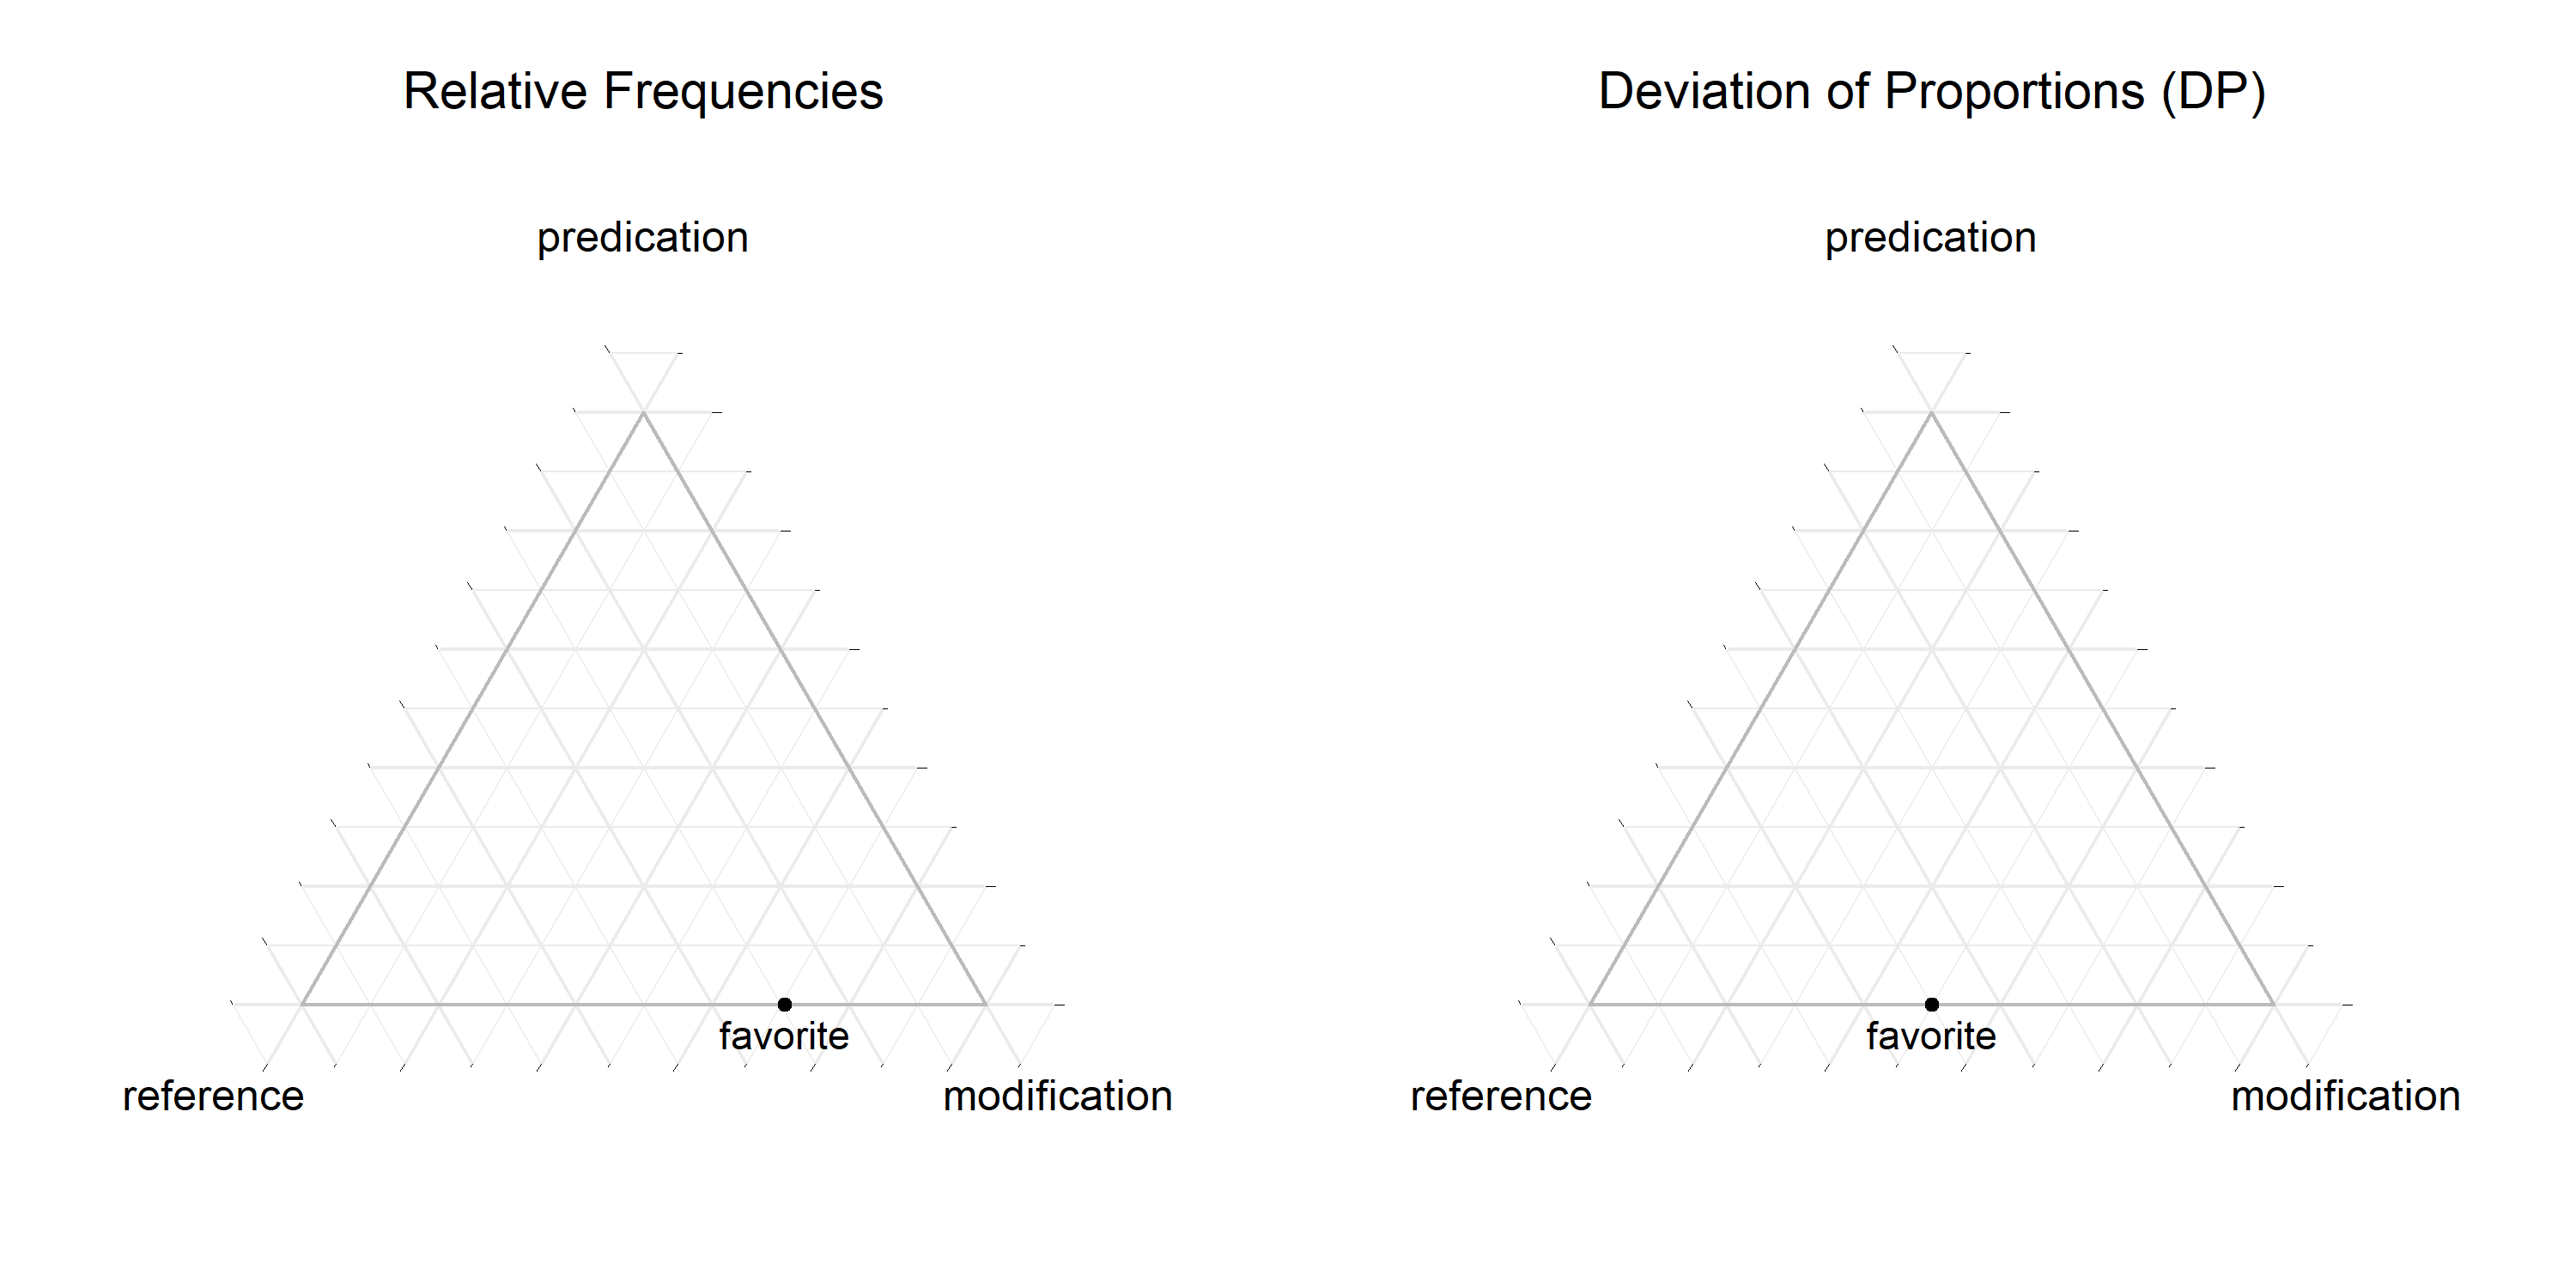
\includegraphics{Eng-favorite-comparison.png}

  \begin{tabular}{ c c c c c c c c c }
    \toprule
    Frequency & Flexibility     & Dispersion & \multicolumn{3}{c}{Frequencies}        & \multicolumn{3}{c}{Dispersions ($DP$)}\\
    { }       & (Shannon's $H$) & ($DP$)     & Reference & Predication & Modification & Reference & Predication & Modification\\
    \midrule
    17        & 0.551           & 0.999      & 5         & 0           & 12           & 0.999     & 1.000       & 0.999       \\
    \bottomrule
  \end{tabular}

\end{figure}
\end{landscape}

\section{R1: Degree of lexical flexibility}
\label{sec:4.3}

In this section I examine the degree of lexical flexibility for words in \idx{English} and \idx{Nuuchahnulth} from several angles, both independently and in comparison, using the lexical flexibility ratings calculated with the methods in \secref*{sec:3.4.1}. The result of these calculations for the 100-item samples are shown in \appref{app:100-item-samples}.

\figref{fig:histogram-100-items} visualizes the distributions of the flexibility ratings for the 100-item samples from \idx{English} (lefthand side) and \idx{Nuuchahnulth} (righthand side). The top portion of each figure is a histogram showing the number of lexical items at different flexibility ratings. Beneath the histograms are boxplots showing the median flexibility rating for each language. \figref{fig:histogram-small-corpus} shows the same visualizations for the small corpus samples.

\begin{figure}

  \centering
  \caption{Distribution of flexibility ratings for the 100-item samples of \idx{English} and \idx{Nuuchahnulth}}
  \label{fig:histogram-100-items}

  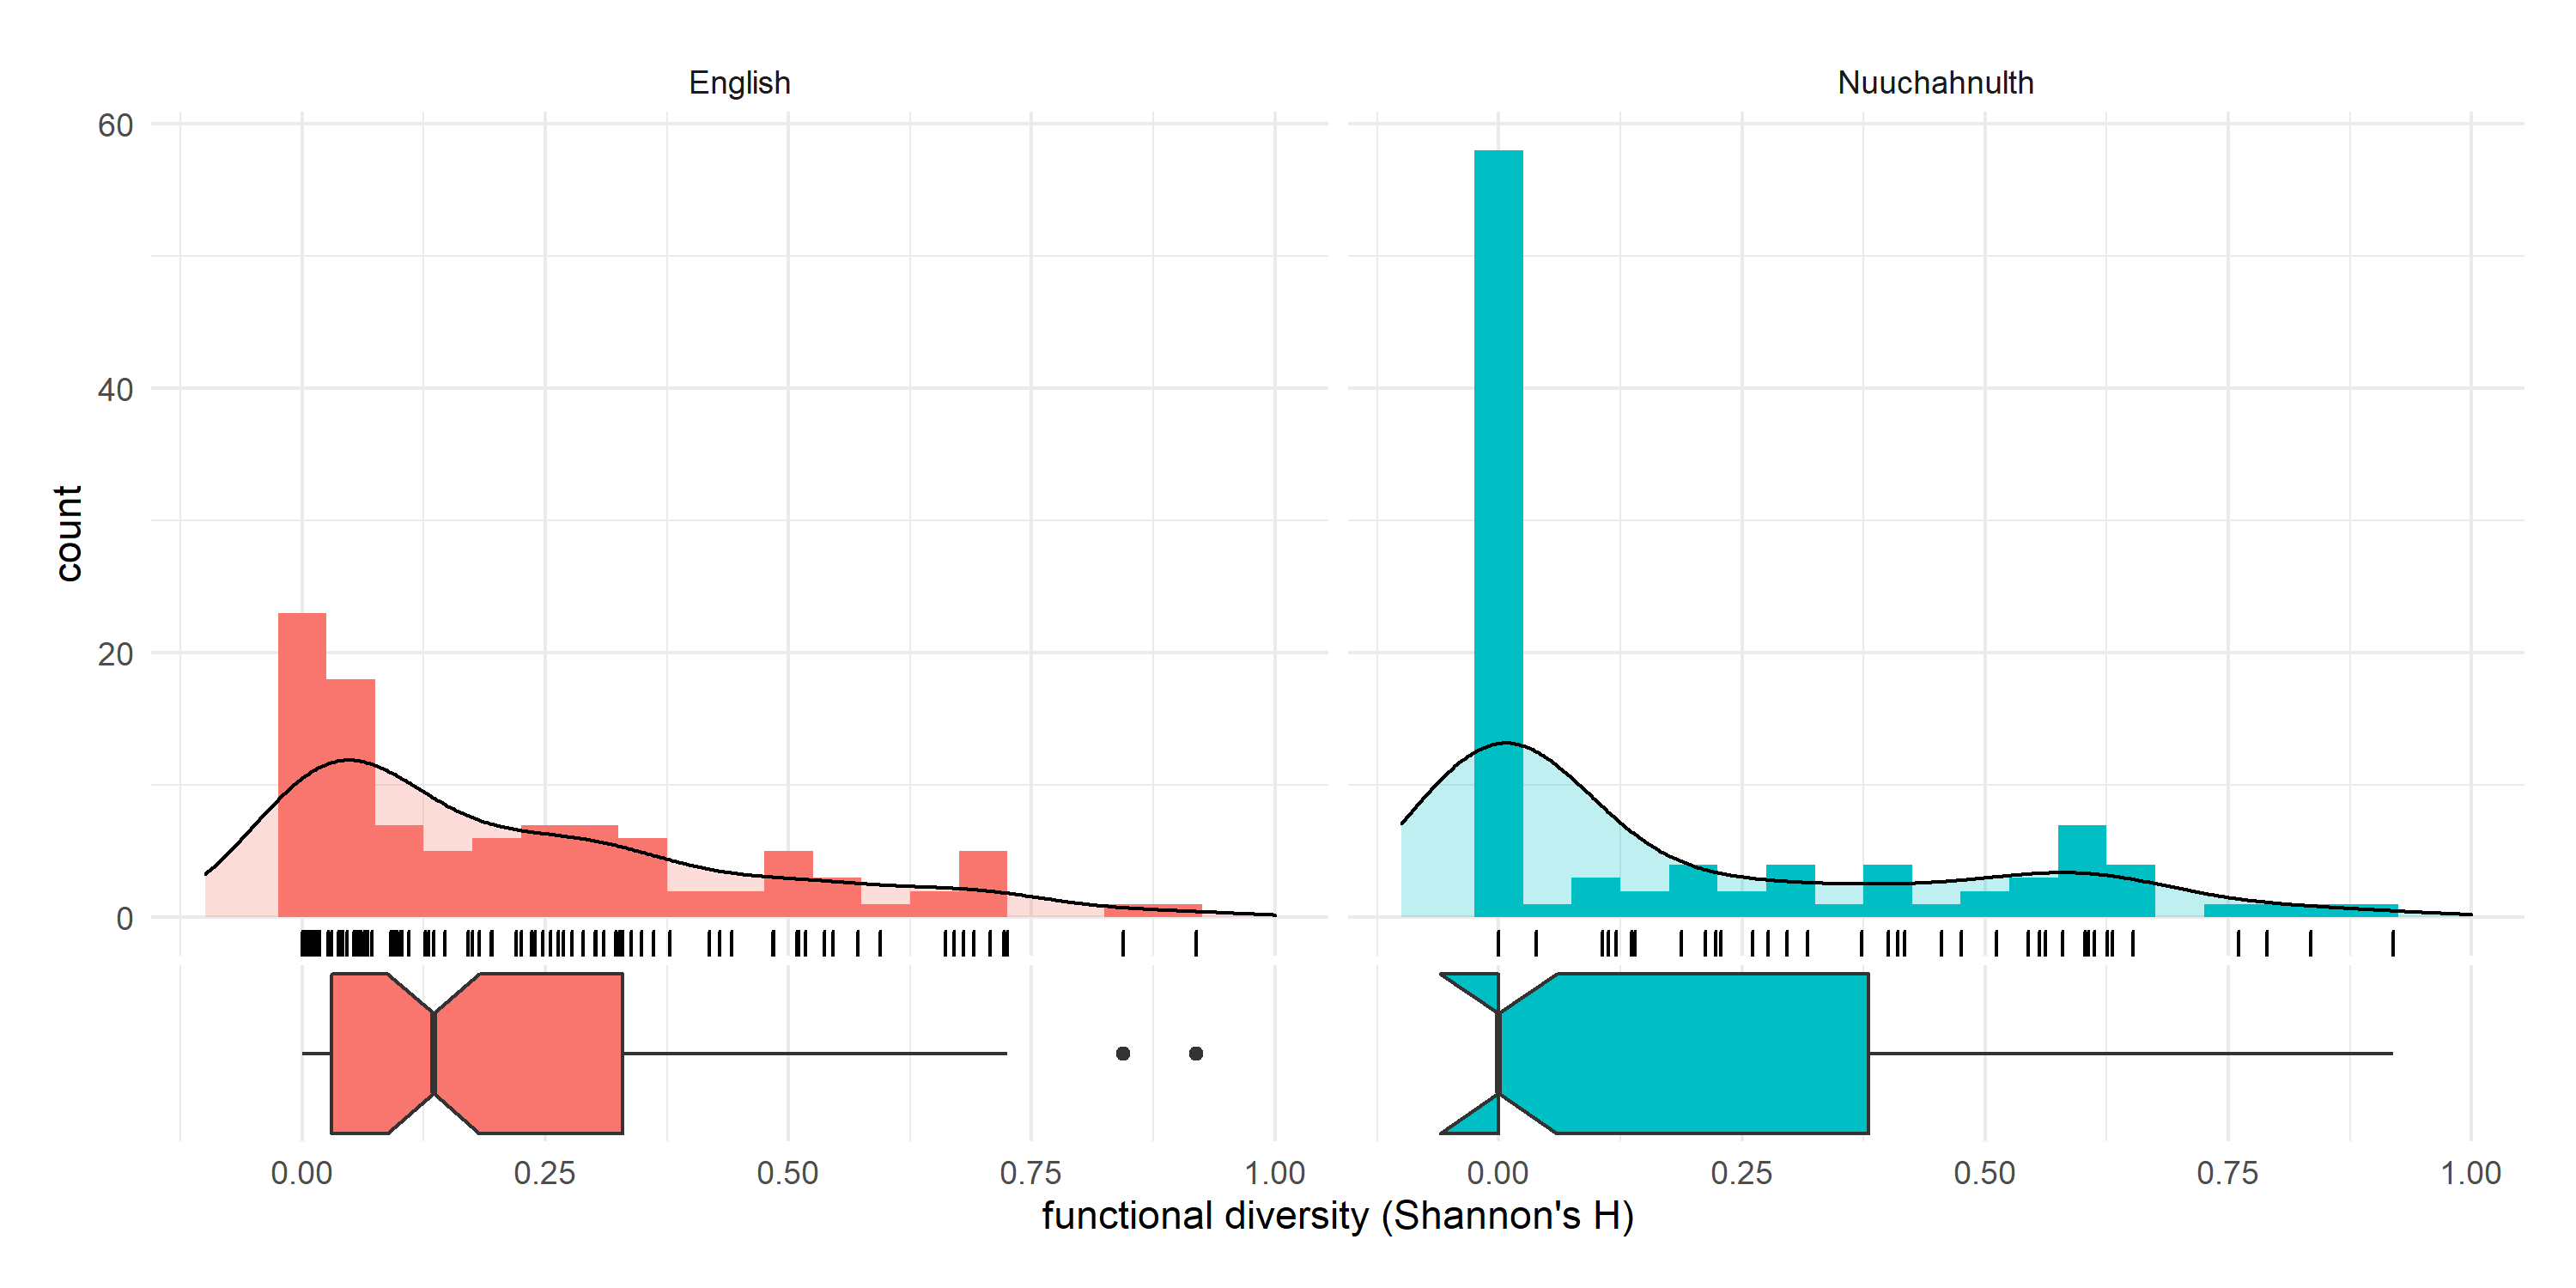
\includegraphics[width=\linewidth]{distribution-100.png}

  \begin{tabular}{ l c c }
    \toprule
    { }                & English & Nuuchahnulth\\
    \midrule
    mean               & 0.223   & 0.183       \\
    median             & 0.134   & 0.000       \\
    standard deviation & 0.230   & 0.259       \\
    \bottomrule
  \end{tabular}

\end{figure}

\begin{figure}

  \centering
  \caption{Distribution of flexibility ratings for the small corpus samples of \idx{English} and \idx{Nuuchahnulth}}
  \label{fig:histogram-small-corpus}

  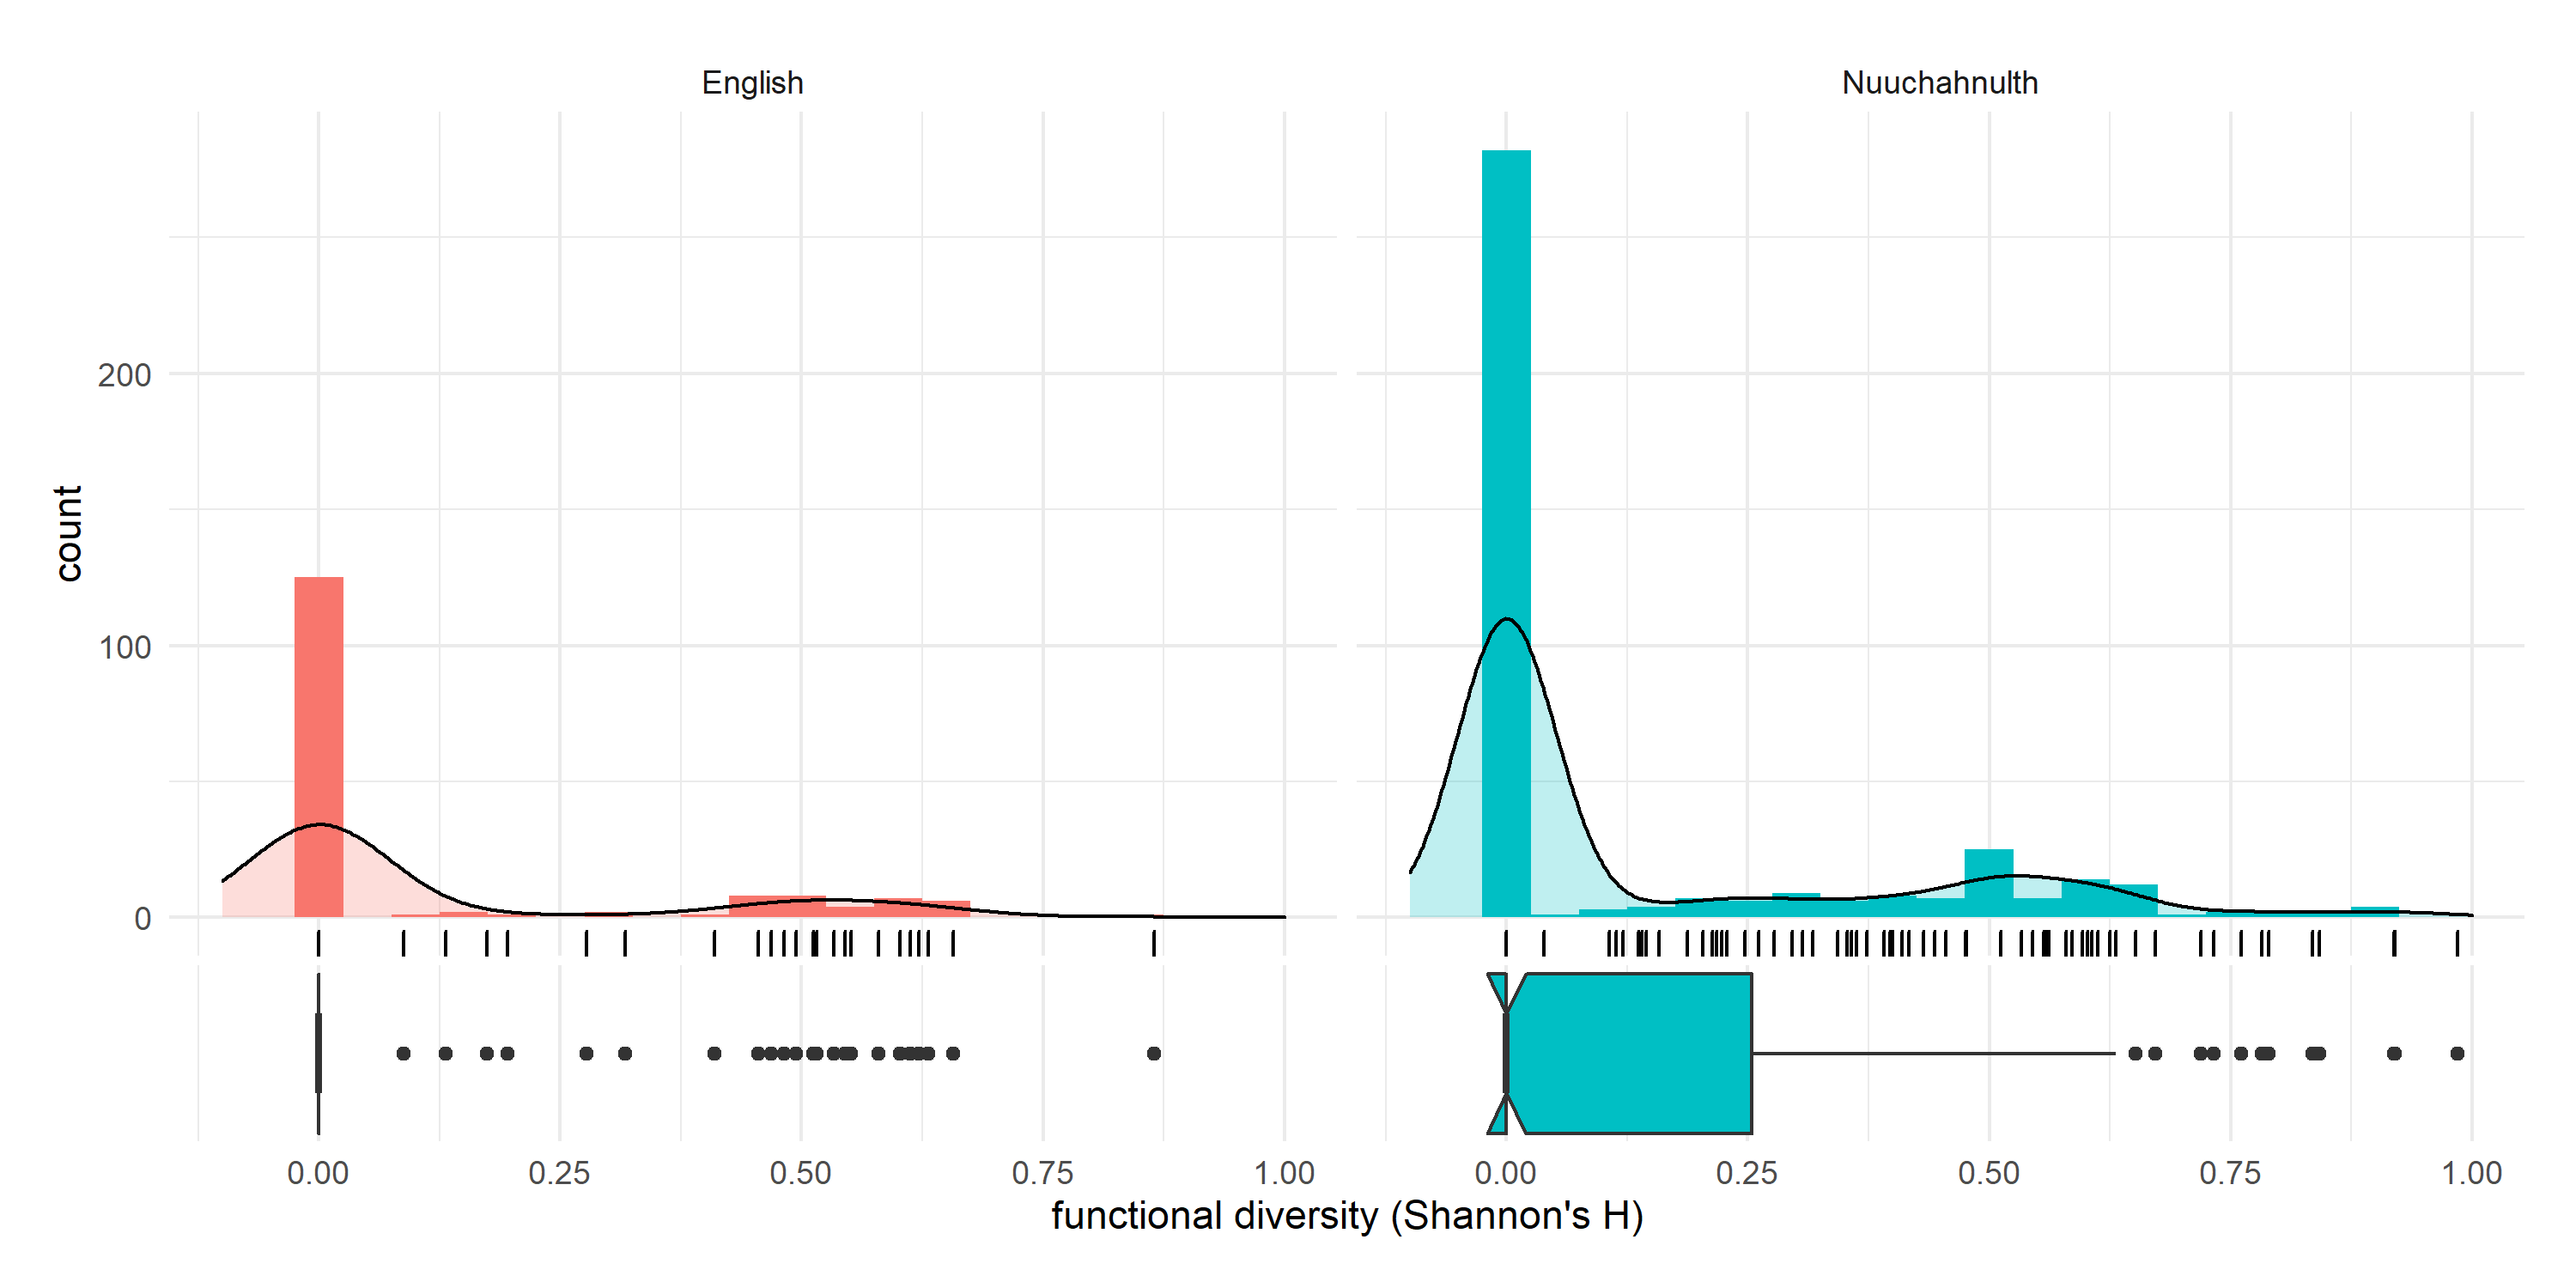
\includegraphics[width=\linewidth]{distribution-small.png}

  \begin{tabular}{ l c c }
    \toprule
    { }                & English & Nuuchahnulth\\
    \midrule
    mean               & 0.122   & 0.143       \\
    median             & 0.000   & 0.000       \\
    standard deviation & 0.226   & 0.243       \\
    \bottomrule
  \end{tabular}

\end{figure}

One immediately obvious observation to be made from these flexibility ratings is that individual lexical items may vary widely in their flexibility, both within and across languages. While this finding is entirely unsurprising, the results very well could have been otherwise. The way \idx{Nuuchahnulth} is often described, one might expect all the lexical items in the language to fall within a more limited range of high-flexibility values. This is clearly not the case. Flexibility ratings for Nuuchahnulth range from the theoretical minimum of $0$ to a maximum of $0.920$ (100-item sample) or $0.985$ (small corpus sample). However, 282 of 483 stems in the small corpus Nuuchahnulth sample (69.97\%) have a flexibility rating of $0$ (58 of stems in the 100-item sample), potentially challenging the claim that all Nuuchahnulth stems are flexible.

Likewise, those who claim that \idx{English} parts of speech are well-defined must confront the fact that the range of flexibility values for English is nearly the same as for \idx{Nuuchahnulth} for both samples: $0$ on the lower end and $.919$ (100-item sample) or $0.865$ (small corpus sample) on the upper end. In fact, in the 100-item samples there are fewer English stems with a flexibility rating of $0$ than there are Nuuchahnulth stems with a flexibility rating of $0$ (8 stems out of 100). The percentage of zero-flexibility stems in the small corpus samples are about equal (125 of 166 stems, or 75.30\%). In this respect, then, English could be viewed as similarly flexible to Nuuchahnulth. Of course, it may be that this difference is due to the large difference in corpus sizes between English and Nuuchahnulth, an issue which is explored in \secref*{sec:4.4}.

Thus the answer to the question, \enquote{Are some lexical items more flexible than others?} is unsurprisingly \enquote{yes}. To pose a related question, \enquote{Can it be shown empirically and quantitatively that some lexical items are more flexible than others, as many linguists have claimed?}. The answer is again, \enquote{yes}. If we want to evaluate the claim that some languages are more or less flexible than others, it must be possible to quantify that flexibility at the level of the individual lexical item and compare them in a meaningful way. The data and methods in this dissertation show that this is indeed possible, and that we can provide clear empirical answers to these kinds of questions. The flexibility of individual lexical items varies widely both within and between languages.

A slightly different question than whether individual stems vary in their flexibility is whether they exhibit flexibility to any substantive degree in the first place. Or, to invert the question, is lexical flexibility a marginal / rare phenomenon which has merely been given disproportionate attention in the literature? A quick look at the flexibility data above shows that this is not the case. When lexical items in \idx{English} and \idx{Nuuchahnulth} exhibit flexibility, it is typically not to a marginal degree. A stem is more likely to have a flexibility of, say, $.200$ than something like $.002$. According to one-sided, one-sample sign tests, the median flexibility in all samples differs highly significantly from zero (see the summary table in \tabref{tab:English-vs-Nuuchahnulth-median}).

\begin{table}
  \centering
  \caption{One-sided, one-sample sign tests for deviation from zero for each corpus sample}
  \label{tab:English-vs-Nuuchahnulth-median}
  \begin{tabular}{ l r l }
    \toprule
    sample                    & V    & p-value\\
    \midrule
    English 100 items         & 4371 & p < .0001\\
    Nuuchahnulth 100 items    & 903  & p < .0001\\
    English small corpus      & 861  & p < .0001\\
    Nuuchahnulth small corpus & 7381 & p < .0001\\
    \bottomrule
  \end{tabular}
\end{table}

This result may seem obvious, but it must be recognized that the result could have been different. Flexibility for \idx{English} stems could have been so marginal as to not significantly deviate from zero. This would have supported an analysis of lexical flexibility in English as mere occasional language play, something exceptional rather than rampant or productive. The data show otherwise: lexical flexibility is a prevalent feature of both English and \idx{Nuuchahnulth}, though to different degrees.

Another question to ask of these data is whether \idx{English} and \idx{Nuuchahnulth} differ in their overall flexibility. The answer to this is not immediately obvious, given how similar the mean and median flexibility ratings for English and Nuuchahnulth are in \figref{fig:histogram-100-items} and \figref{fig:histogram-small-corpus}. But to reduce the entire lexicon of a language to a single measure of central tendency obscures important details. The \emph{way} in which the two languages exhibit flexibility is arguably more interesting.

How then is lexical flexibility realized in \idx{English} and \idx{Nuuchahnulth}? In addition to the histograms in \figref{fig:histogram-100-items} and \figref{fig:histogram-small-corpus}, the ternary plots in \figref{fig:ternary-100-items} and \figref{fig:ternary-small-corpus} illustrate the way that flexibility operates in these two languages. In these figures, each lexical item is represented by a single point on the ternary plot.

\begin{figure}[h!]
  \centering
  \caption{Distribution of functions for the 100-item samples of \idx{English} and \idx{Nuuchahnulth}}
  \label{fig:ternary-100-items}
  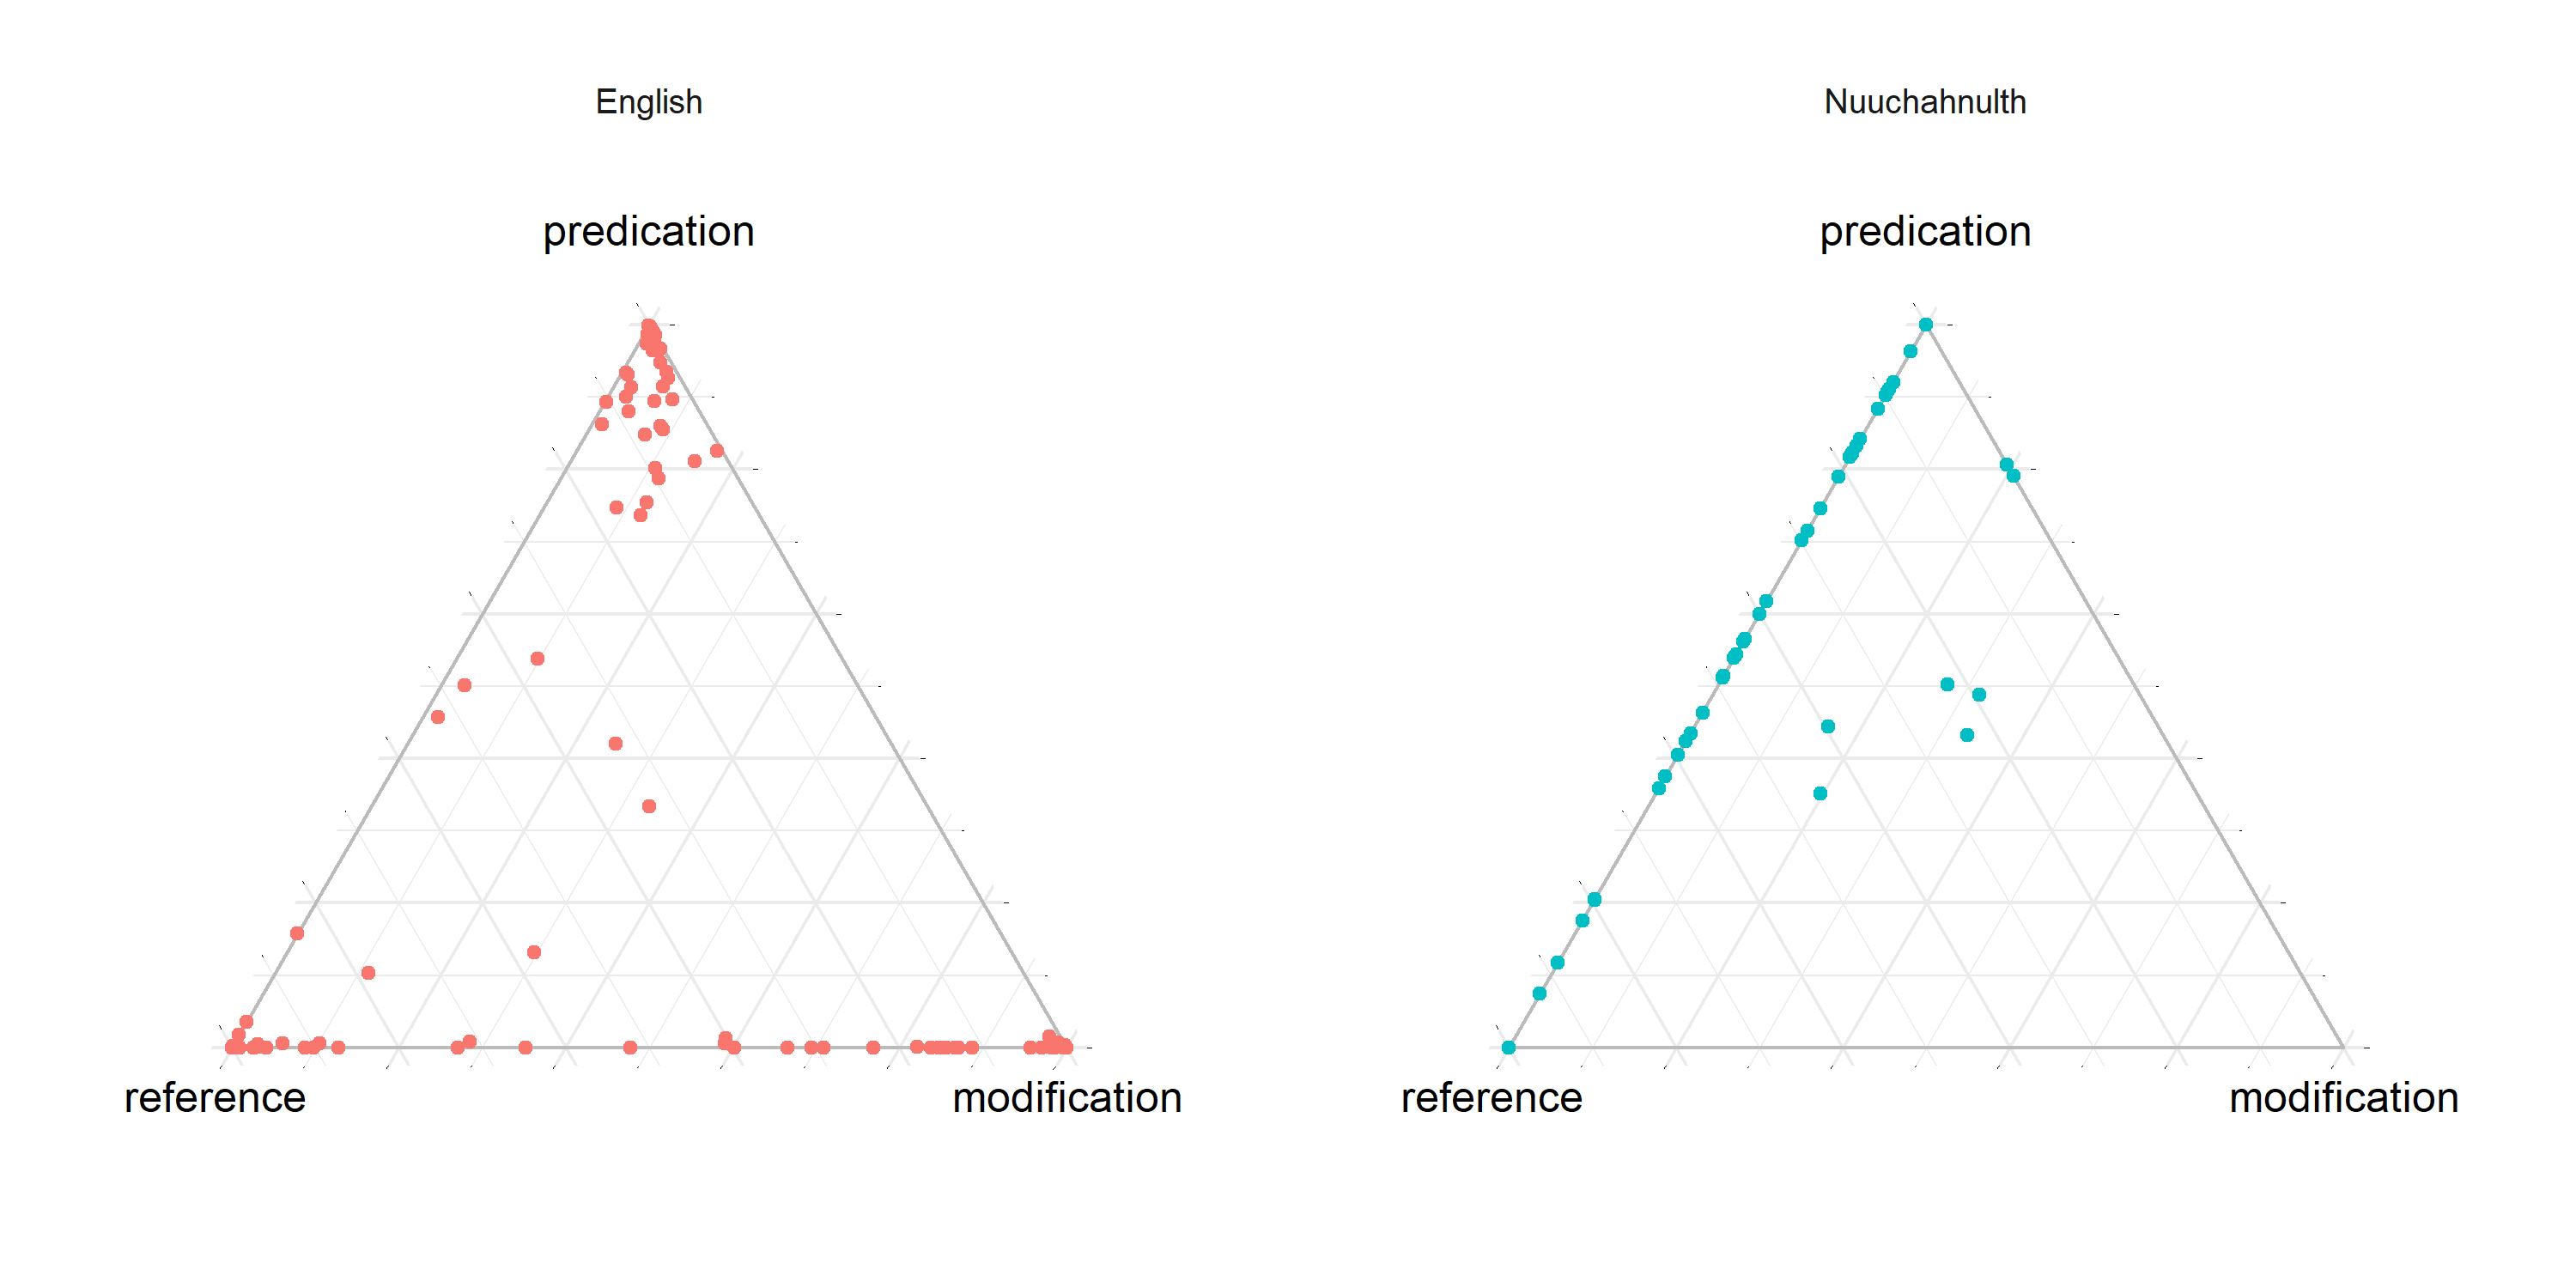
\includegraphics[width=\linewidth]{functions-100.png}
\end{figure}

\begin{figure}[h!]
  \centering
  \caption{Distribution of functions for the small corpus samples of \idx{English} and \idx{Nuuchahnulth}}
  \label{fig:ternary-small-corpus}
  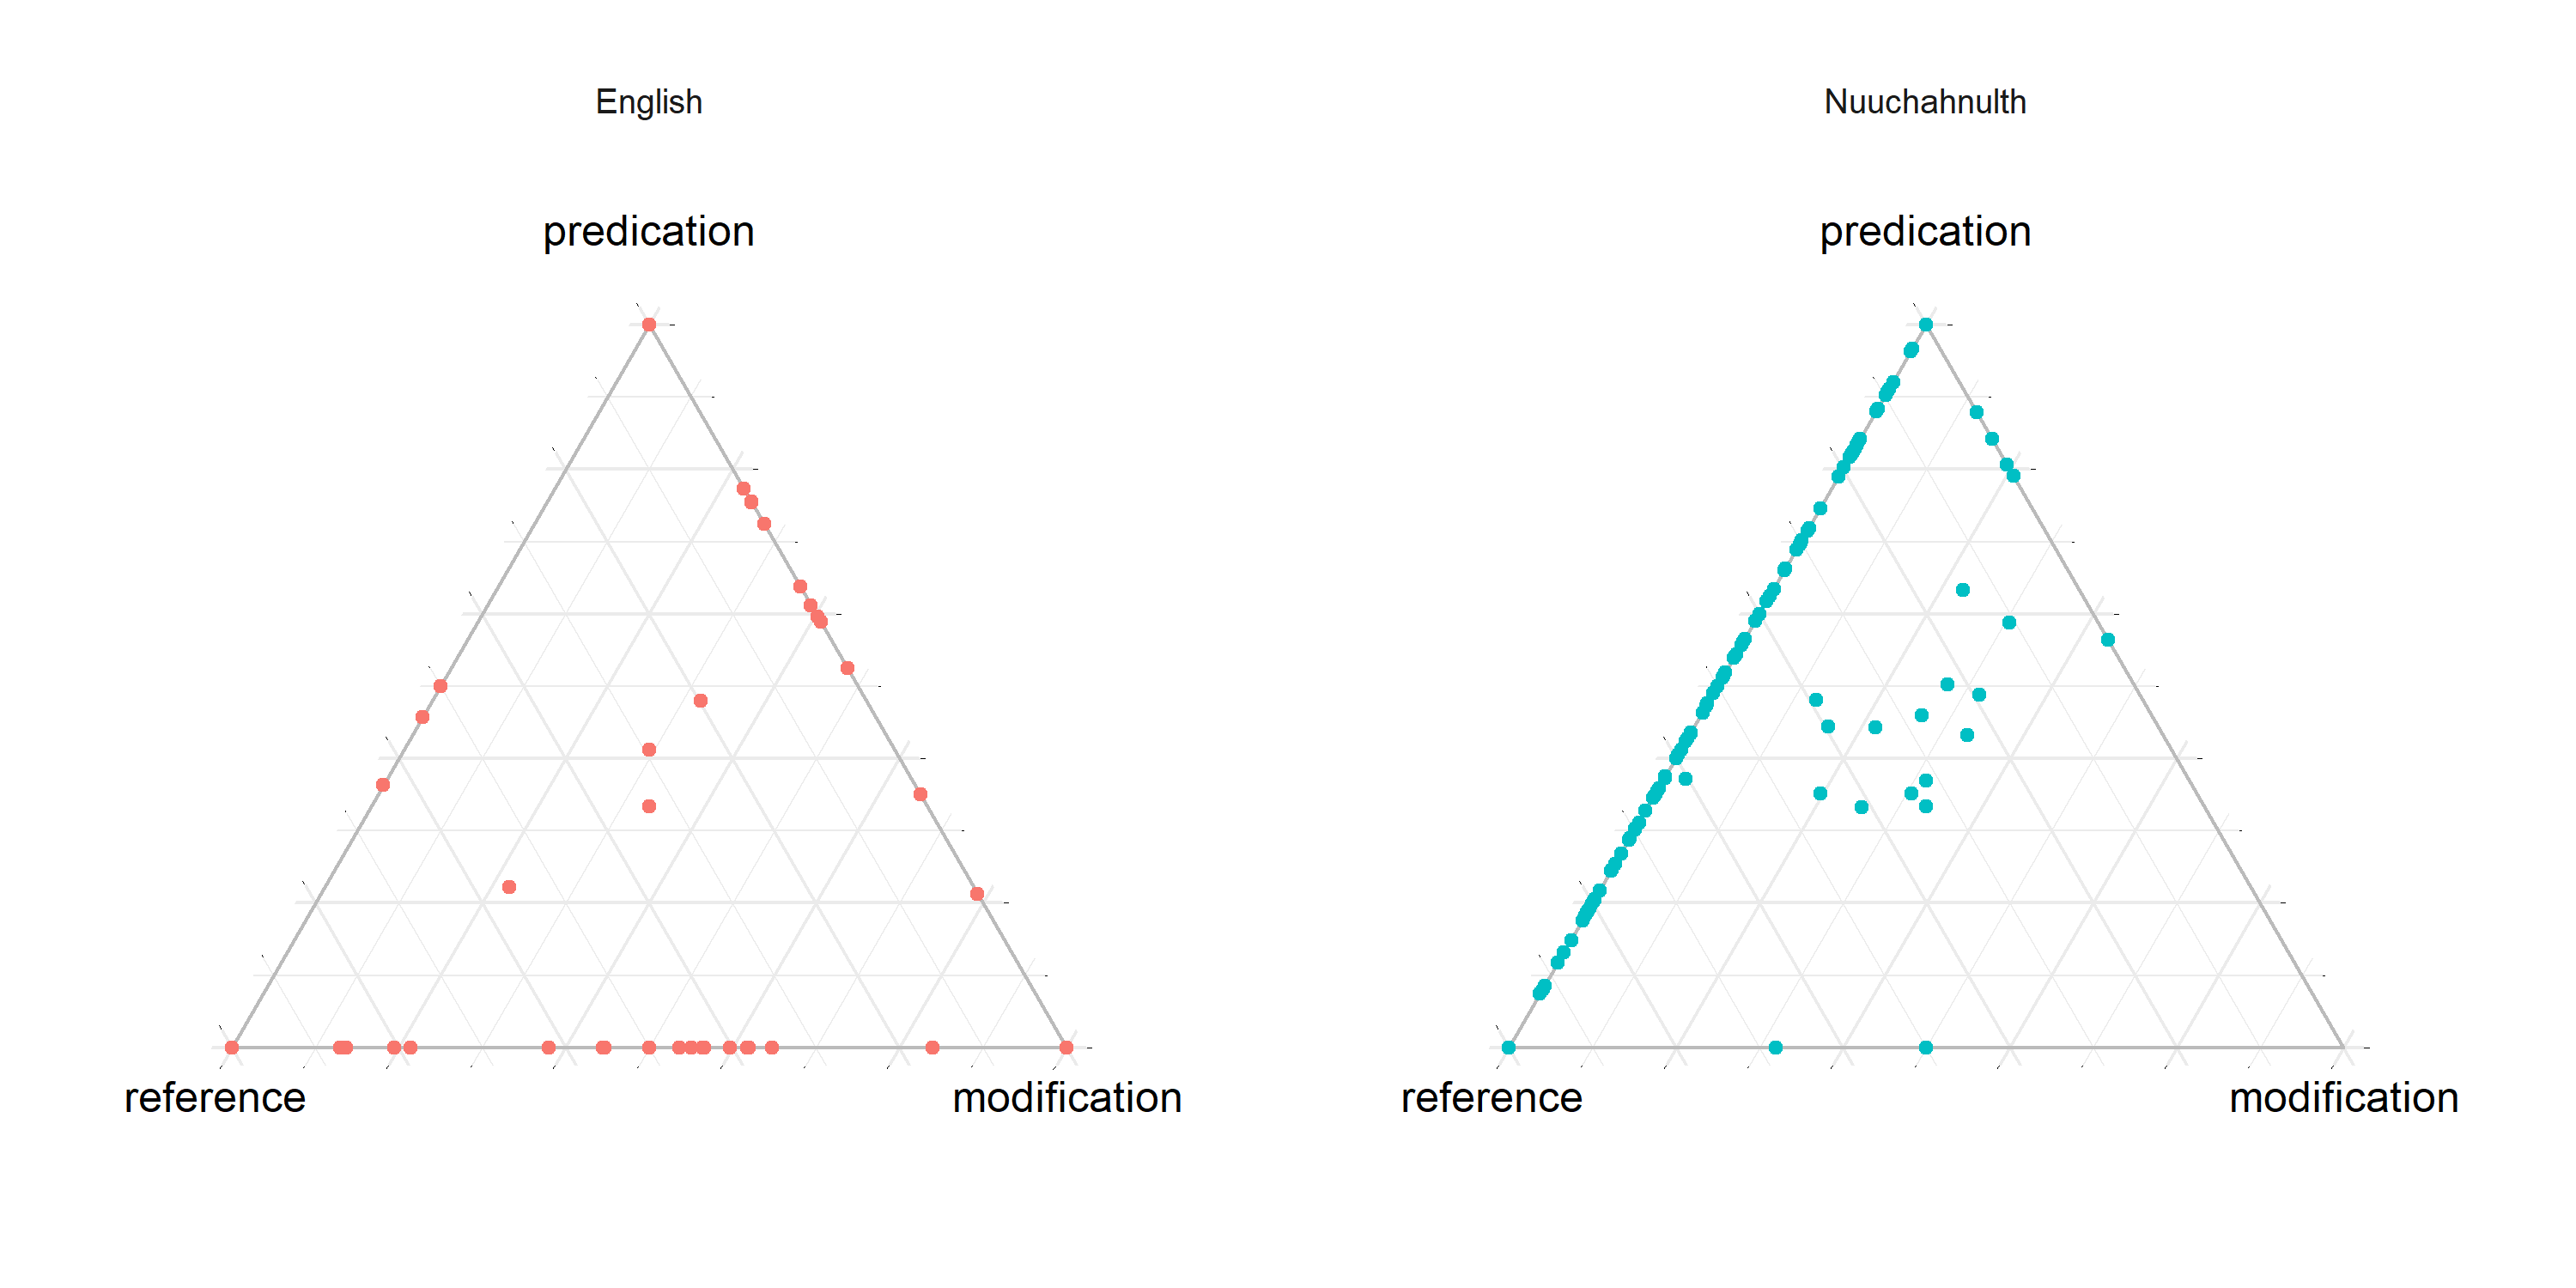
\includegraphics[width=\linewidth]{functions-small.png}
\end{figure}

Beginning with \idx{English}, we can see that most lexical items exhibit some flexibility, but to a relatively small degree. After zero-flexibility cases, the next most frequent flexibility rating is in the $0$–$0.05$ range. This is also evident from the ternary plots, where lexical items tend to cluster near (but not precisely on) the corners for their most prototypical functions. Interestingly, the small English corpus appears to show \emph{more} flexibility than the 100-item sample. This could be an effect of the specific words chosen, but it could also be the case that it takes a certain number of tokens for the prototypical function of an item to become evident. This possibility is examined further in \secref*{sec:4.4}.

\idx{Nuuchahnulth} differs from English in several notable ways. First, a much higher proportion of items display no flexibility whatsoever. However, for those items which do exhibit flexibility, the average flexibility rating is generally higher than that of English stems. In both samples, the biggest cluster of items with non-zero flexibility ratings have ratings around $.6$. English items with non-zero flexibility, by comparison, generally have ratings closer to $.2$. Thus for Nuuchahnulth lexical items are either totally inflexible or generally strongly flexible.

This bifurcation of the data is very likely due to the small size of the \idx{Nuuchahnulth} corpus, as will be discussed in \secref*{sec:4.4}. It may be that Nuuchahnulth words are generally highly flexible, but that more tokens are needed to see this trend. Alternatively, it may be that certain Nuuchahnulth stems are strongly associated with a specific discourse function and thus inflexible, while others are generally flexible. This would suggest a probabilistic division of Nuuchahnulth stems into two classes: those that are productively flexible, and those that are not.

This second possibility would challenge existing analyses of \idx{Nuuchahnulth}. The existence of a productively flexible class of stems would be counterevidence to the many claims that Nuuchahnulth word classes can in fact be clearly defined using selectional criteria such as ability to take possession or the definite suffix \parencites{Jacobsen1979}{DavisGillonMatthewson2014}{Braithwaite2015}. Similarly, \textcite[57]{Nakayama2001} characterizes word classes in Nuuchahnulth as strong statistical tendencies in discourse. For many Nuuchahnulth stems, however, there is no clear prototypical use. The data show that many stems are used roughly equally for predication as they are for reference, making it difficult to assess which use is more basic or unmarked.

As the ternary plots for \idx{Nuuchahnulth} in \figref{fig:ternary-100-items} and \figref{fig:ternary-small-corpus} make clear, the distribution of lexical items across functions in Nuuchahnulth differs strongly from that of English. For starters, there is very little clustering around prototypical functions in the corners, in direct contrast to English. Secondly, Nuuchahnulth shows very little flexibility in the modification direction, but rampant flexibility along the reference-predication axis. For the small corpus sample in particular, there is a smooth cline of values between reference and predication. Nuuchahnulth stems sit anywhere on a continuum from prototypical referents to prototypical predicates, but none show prototypical modifier behavior.

These findings nicely reflect the intuitions of many researchers about these two languages. \idx{English} is mostly rigid, but most words exhibit a marginal degree of flexibility. English words are \emph{primarily} associated with one discourse function, but not exclusively so. \idx{Nuuchahnulth}, by contrast, shows a very high degree of reference-predicate flexibility. However, Nuuchahnulth stems are not frequently used for modification. This is in line with the analysis of most researchers regarding lexical categories in Nuuchahnulth. \textcite[50]{Nakayama2001}, for example, says that the categories noun and verb must be recognized for Nuuchahnulth, but that there is not sufficient evidence to justify an adjective category, even as a statistical tendency. He instead treats \enquote{adjectivals} as a subclass of verbs. The central location of the points in the Nuuchahnulth plot in \figref{fig:ternary-small-corpus}, however, suggest that Nuuchahnulth modifiers are as nounlike as they are verblike. The low frequency with which stems are used for modification also mirrors the results from \posscitet[88--89]{Croft1991} four-language survey of the textual frequency of different lexical classes. He also finds that \textquote[{\cite[88--89]{Croft1991}}]{the overall frequency of roots denoting properties and occurrences of modifiers is extremely low compared to the frequencies of object and action roots and of referring expressions and predications}.

\section{R2: Lexical flexibility and corpus size}
\label{sec:4.4}

It seems intuitively plausible that the more tokens of a word one encounters, the more likely one is to find flexible uses of a word. With a large enough corpus, all items would exhibit flexibility. This has been claimed by \textcite[77]{MoselHovdhaugen1992}. It may be the case that larger corpora are statistically more flexible than smaller corpora. However, to my knowledge this claim has never been tested empirically, although the fact that the median flexibility for the small corpus sample of \idx{English} is $0$ while the median flexibility of the much larger 100-item sample is $0.134$ suggests that the hypothesis might be true. In this section I examine the results of comparing the number of tokens encountered for a stem to its cumulative flexibility rating, the question being, \enquote{Does the cumulative flexibility for the lexical item increase as one encounters more tokens?}.

Only stems with a frequency of at least 4 were studied (see \secref{sec:3.4.1} for the motivation behind this restriction). For English, I examined the 100-item sample, and for Nuuchahnulth I used the entire corpus. Using a script and going sequentially through the corpora, each time I encountered a new token of a lexical item, I recalculated its flexibility and recorded that value and token frequency at that point in the corpus.

\figref{fig:cumulative-flexibility-words-English} shows the result of these calculations for the ten most frequent words in the \idx{English} corpus, and \figref{fig:cumulative-flexibility-words-Nuuchahnulth} shows the same for \idx{Nuuchahnulth}. The number of tokens encountered is shown on the x-axis, and the cumulative flexibility is shown on the y-axis. I show only the most frequent words here merely because they provide the clearest visual representation of the data; more comprehensive (but more difficult to read) plots for each language are given in \figref{fig:cumulative-flexibility-all-English} and \figref{fig:cumulative-flexibility-all-Nuuchahnulth}. For ease of visualization, a version of the English data with $\log_{10}$ frequency on the x-axis is also given in \figref{fig:cumulative-flexibility-English-log}.

\begin{figure}[h!]
  \centering
  \caption{Cumulative lexical flexibility for \idx{English} (10 most frequent words)}
  \label{fig:cumulative-flexibility-words-English}
  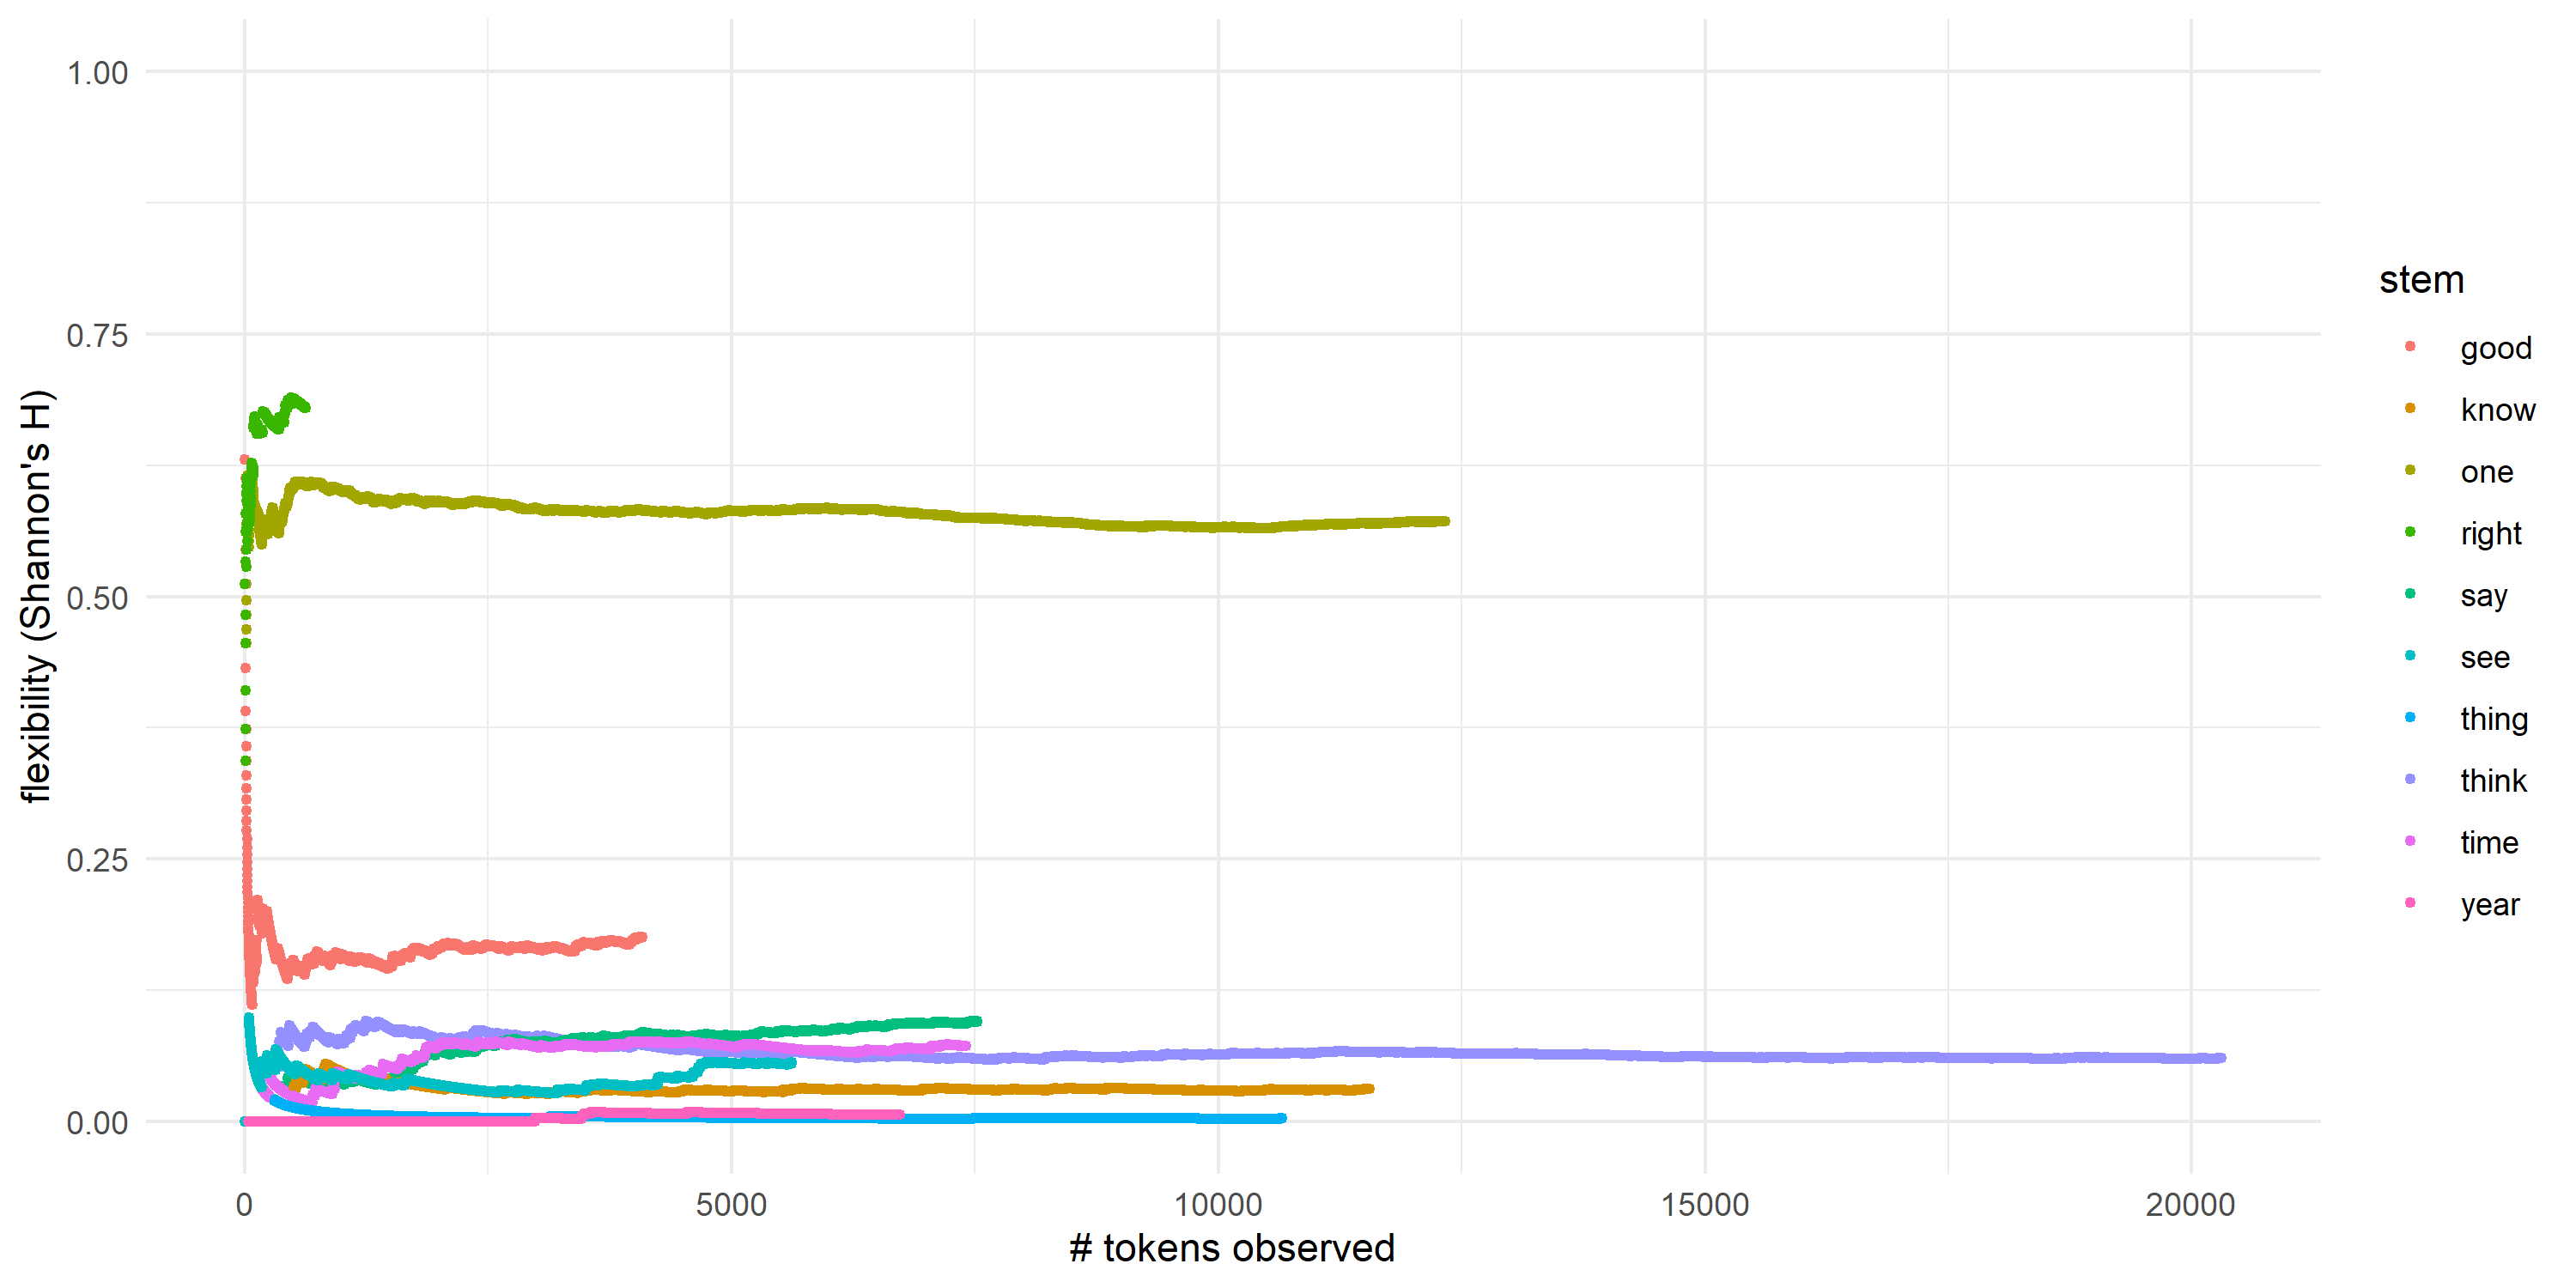
\includegraphics[width=\linewidth]{cumulative-flexibility-words-English.png}
\end{figure}

\begin{figure}[h!]
  \centering
  \caption{Cumulative lexical flexibility for \idx{Nuuchahnulth} (10 most frequent words)}
  \label{fig:cumulative-flexibility-words-Nuuchahnulth}
  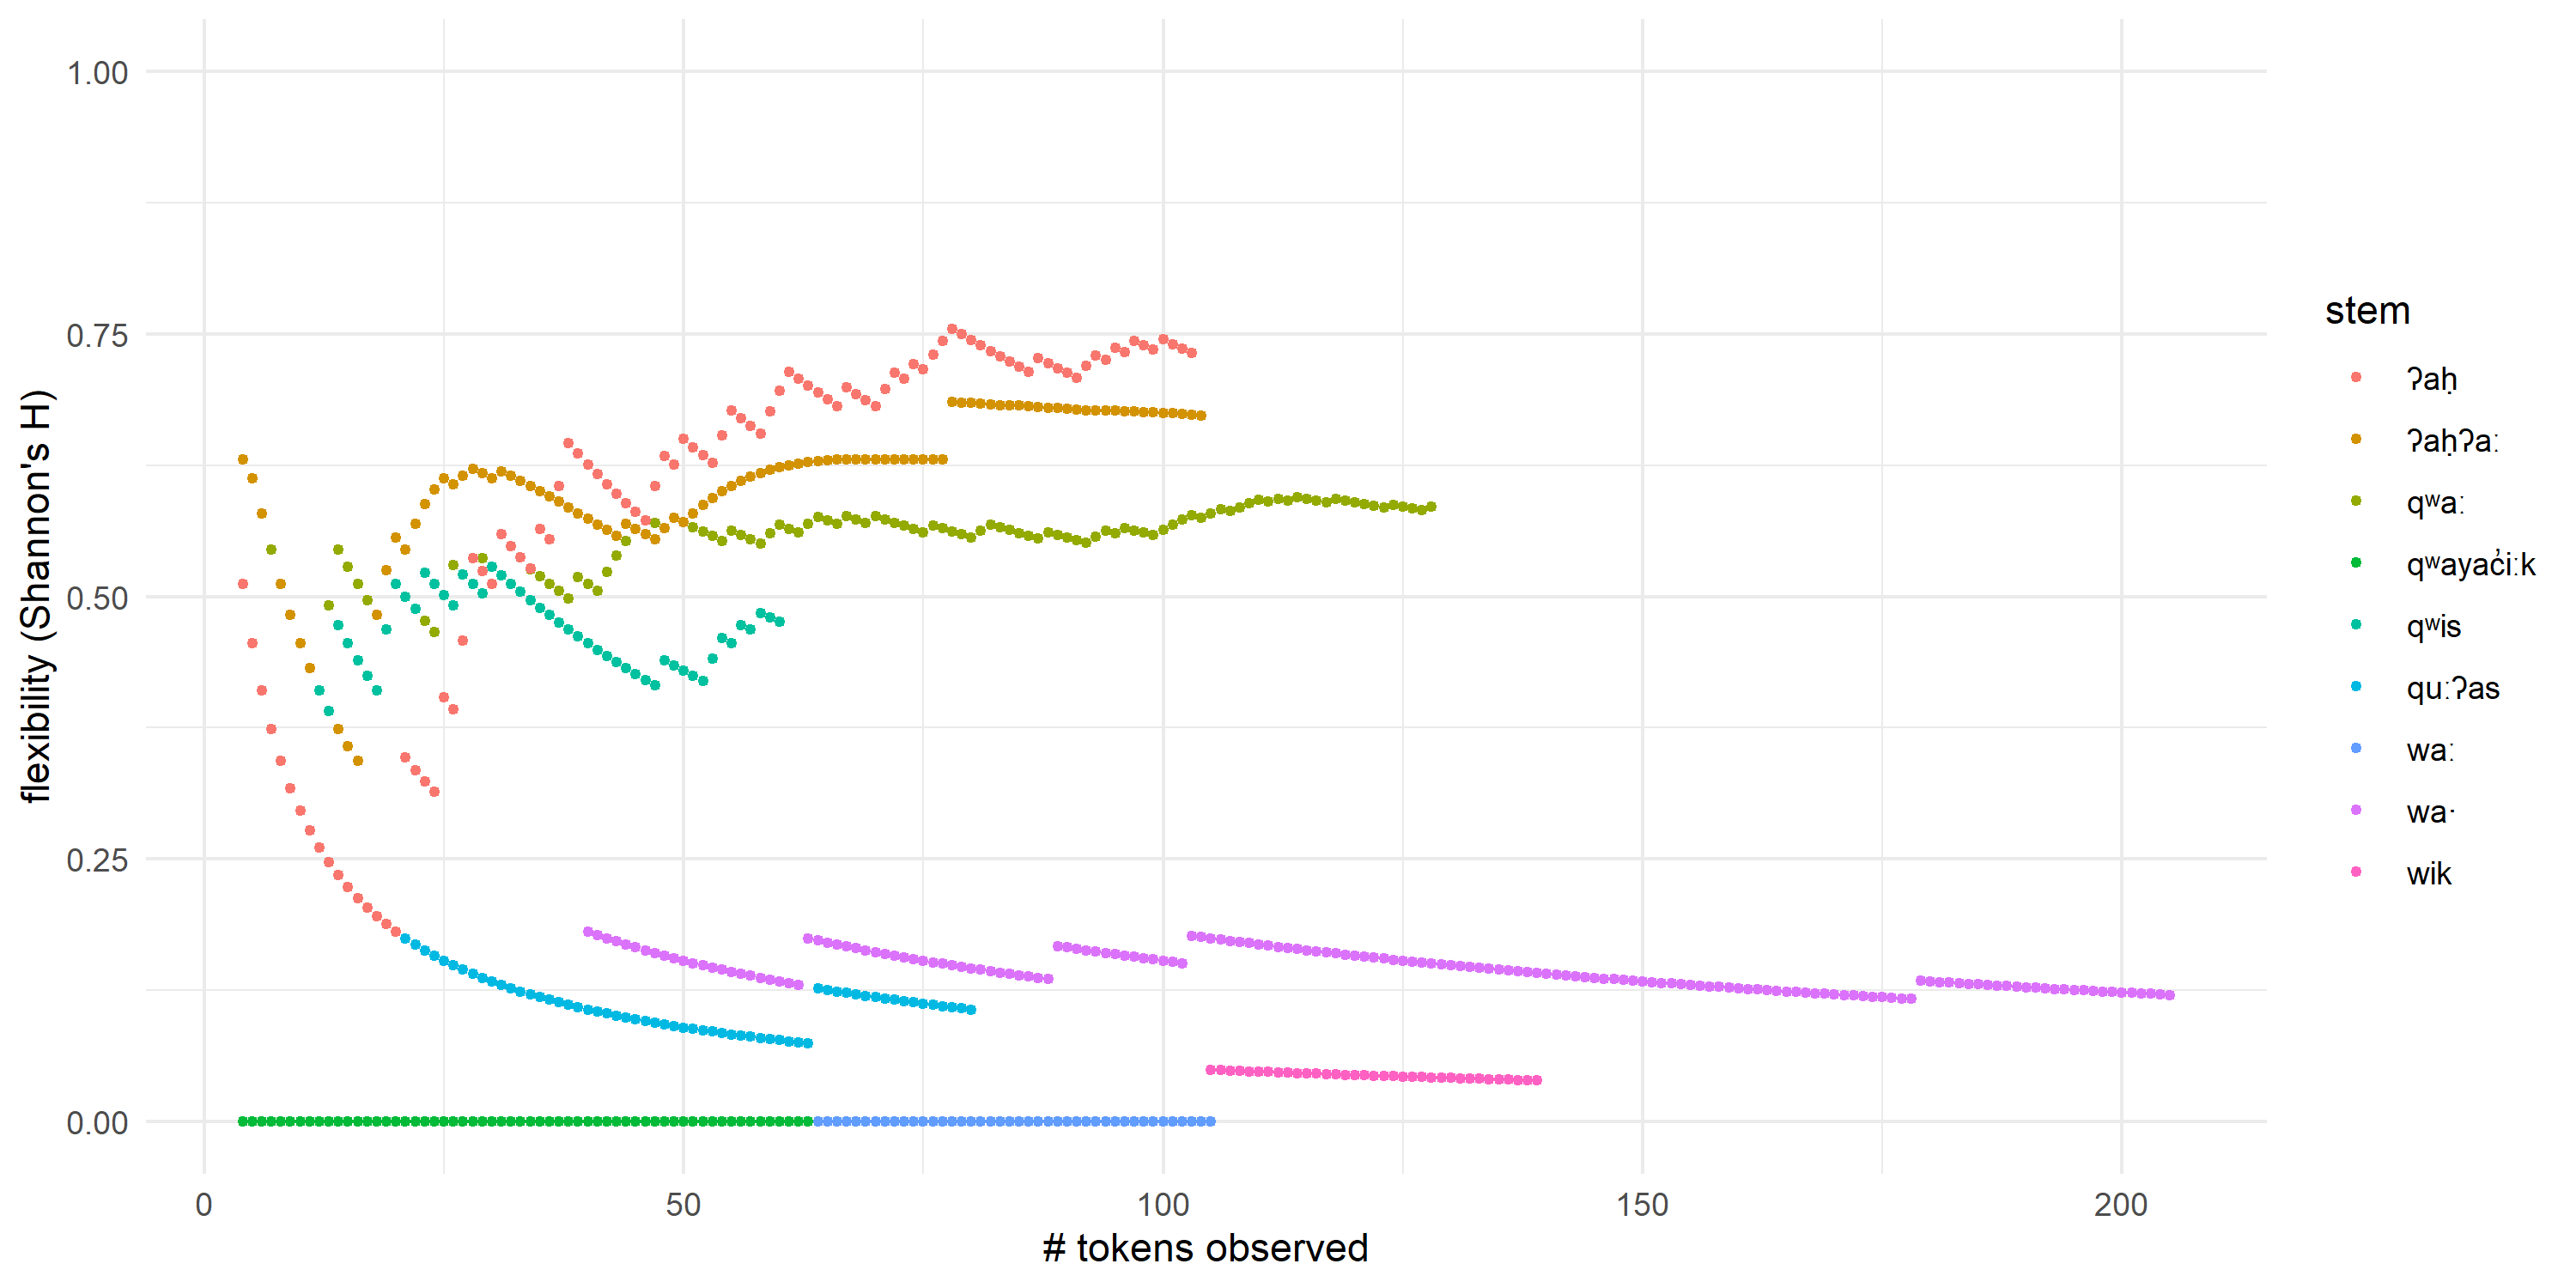
\includegraphics[width=\linewidth]{cumulative-flexibility-words-Nuuchahnulth.png}
\end{figure}

\begin{figure}[h!]
  \centering
  \caption{Cumulative lexical flexibility for \idx{English} (all words)}
  \label{fig:cumulative-flexibility-all-English}
  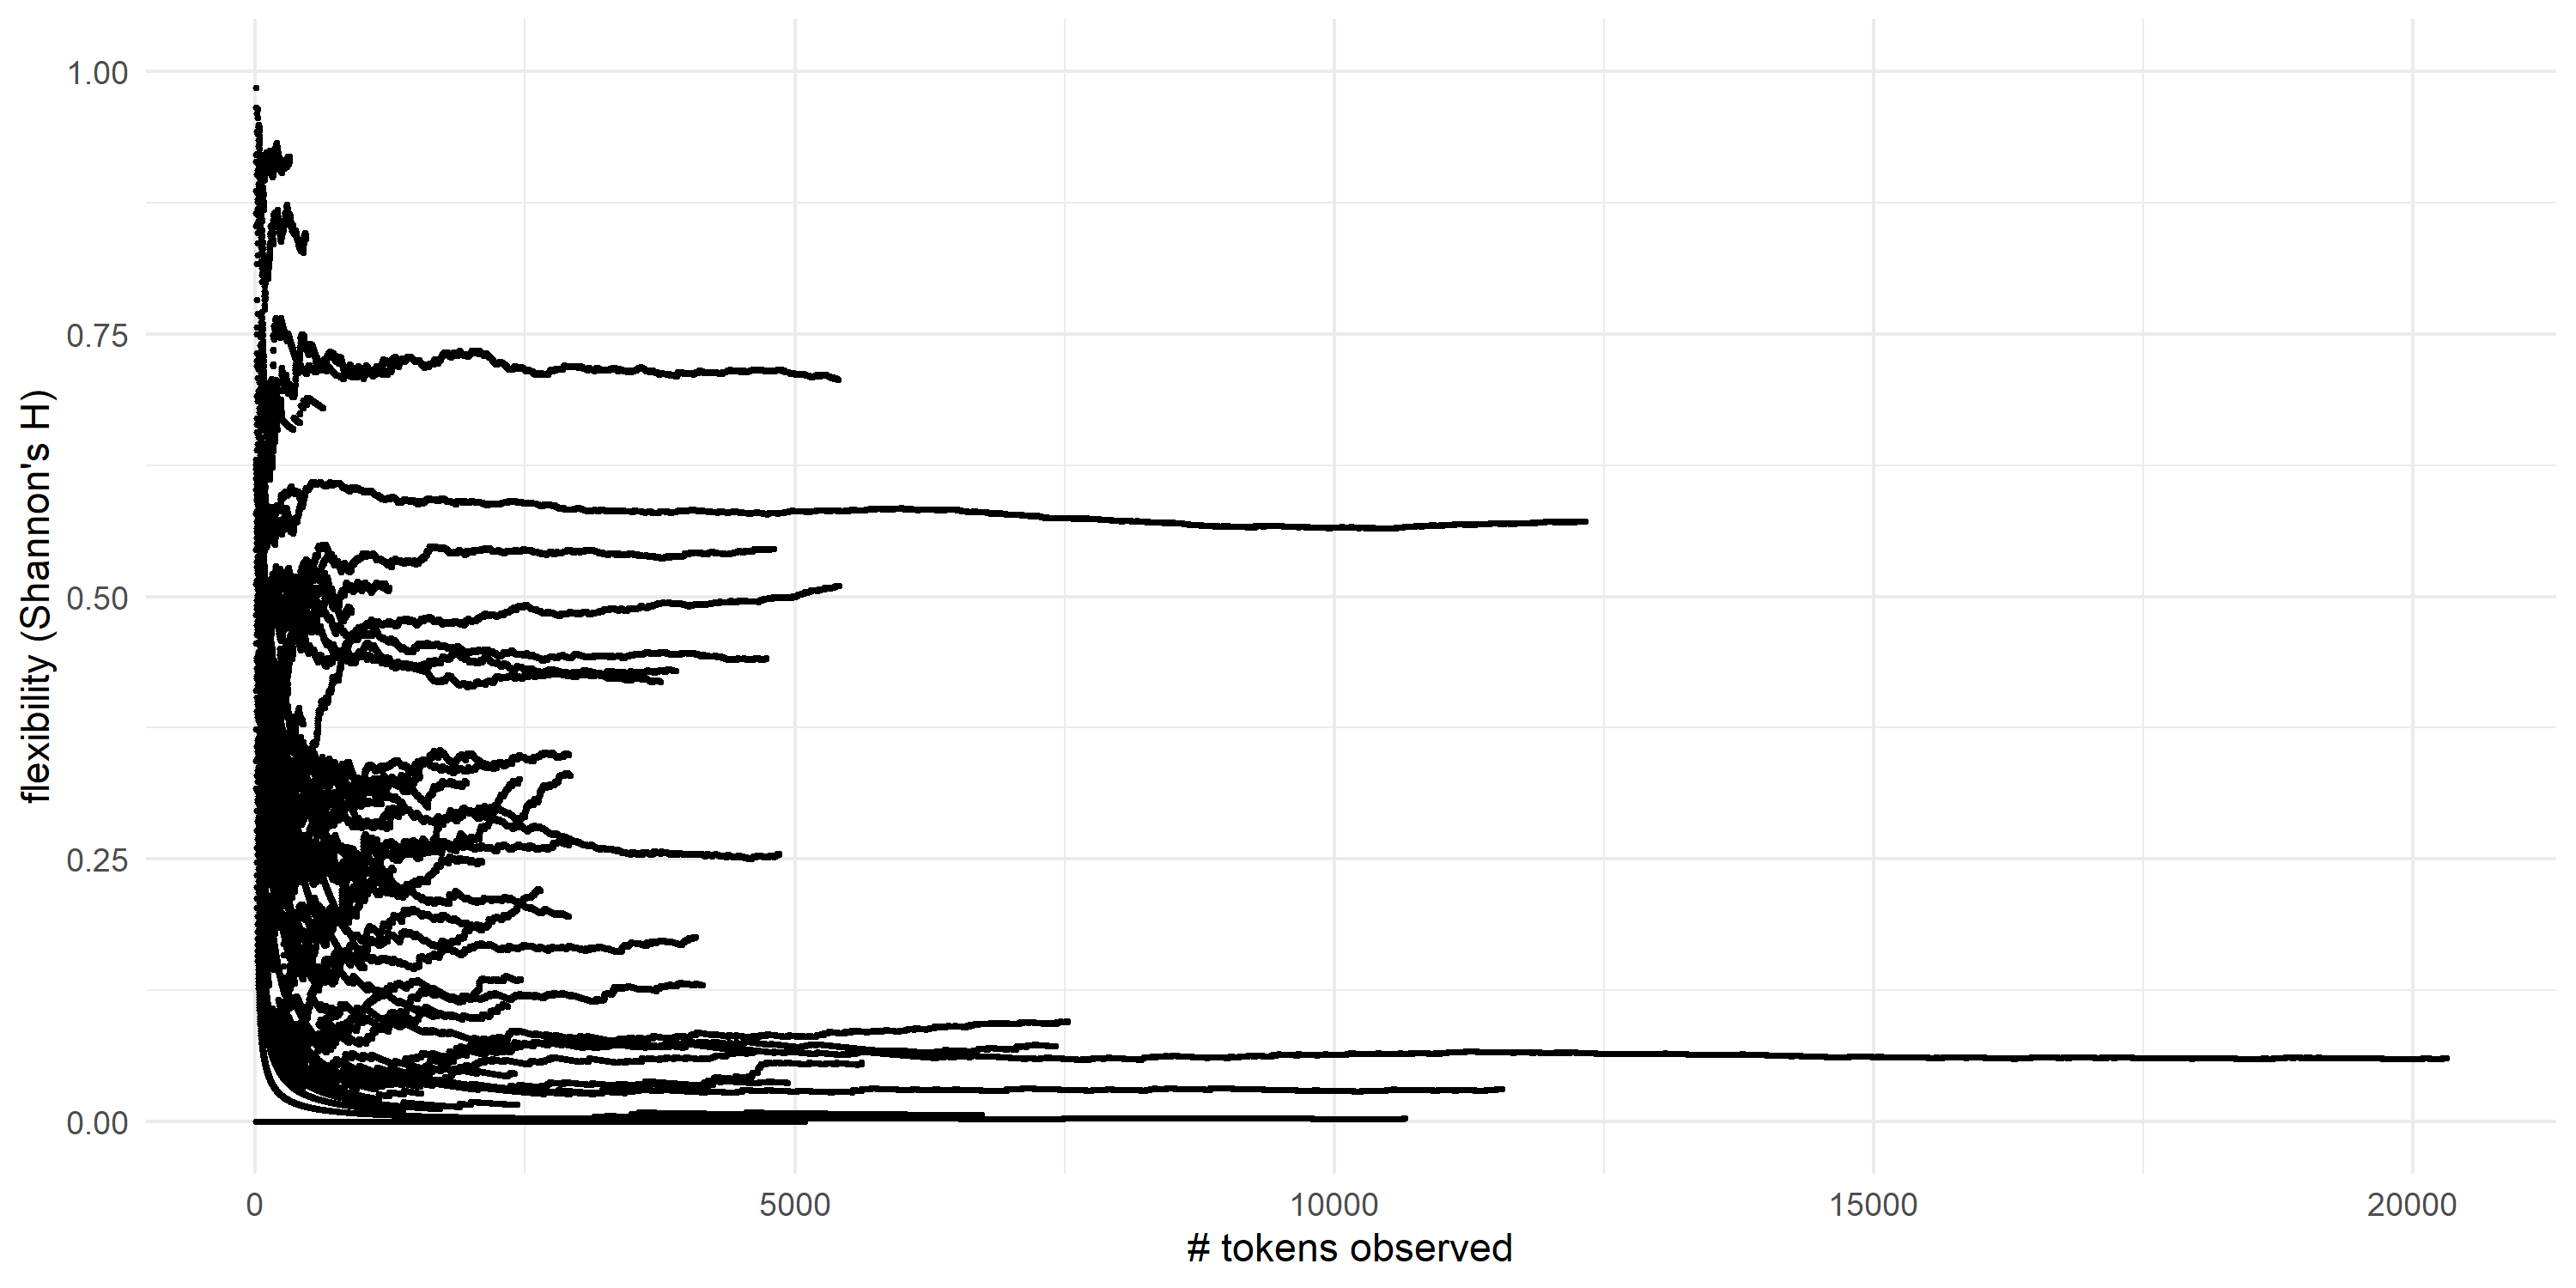
\includegraphics[width=\linewidth]{cumulative-flexibility-all-English.png}
\end{figure}

\begin{figure}[h!]
  \centering
  \caption{Cumulative lexical flexibility for \idx{Nuuchahnulth} (all words)}
  \label{fig:cumulative-flexibility-all-Nuuchahnulth}
  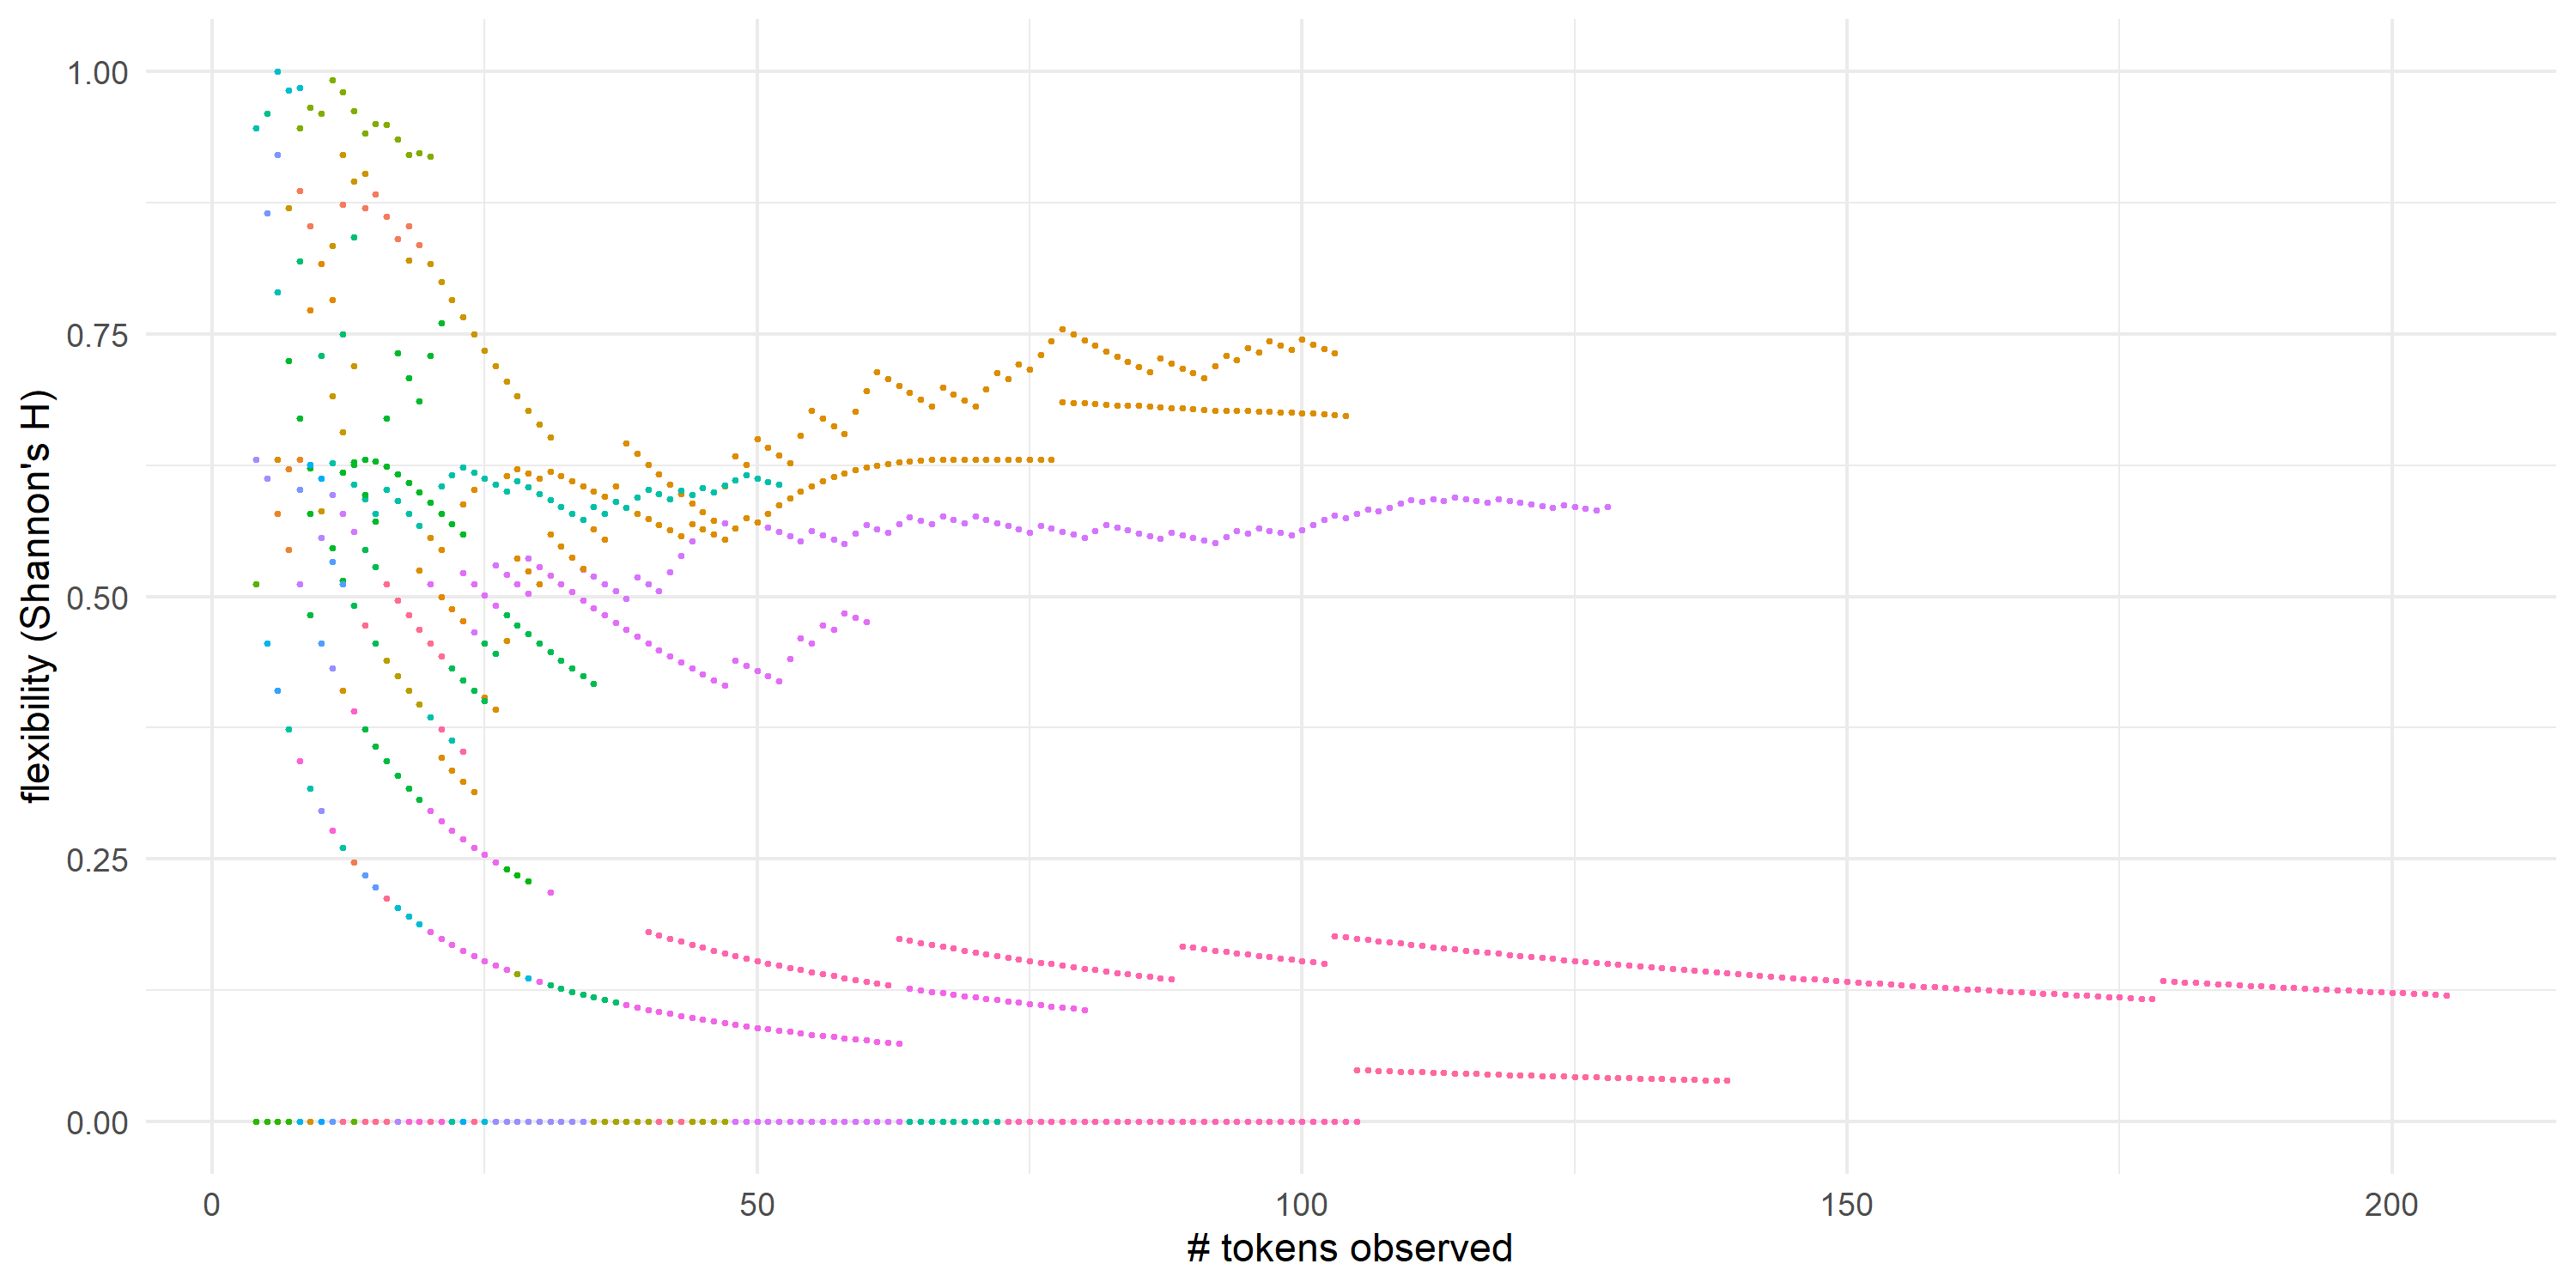
\includegraphics[width=\linewidth]{cumulative-flexibility-all-Nuuchahnulth.png}
\end{figure}

\begin{figure}[h!]
  \centering
  \caption{Cumulative lexical flexibility for \idx{English} ($log_10$ scale)}
  \label{fig:cumulative-flexibility-English-log}
  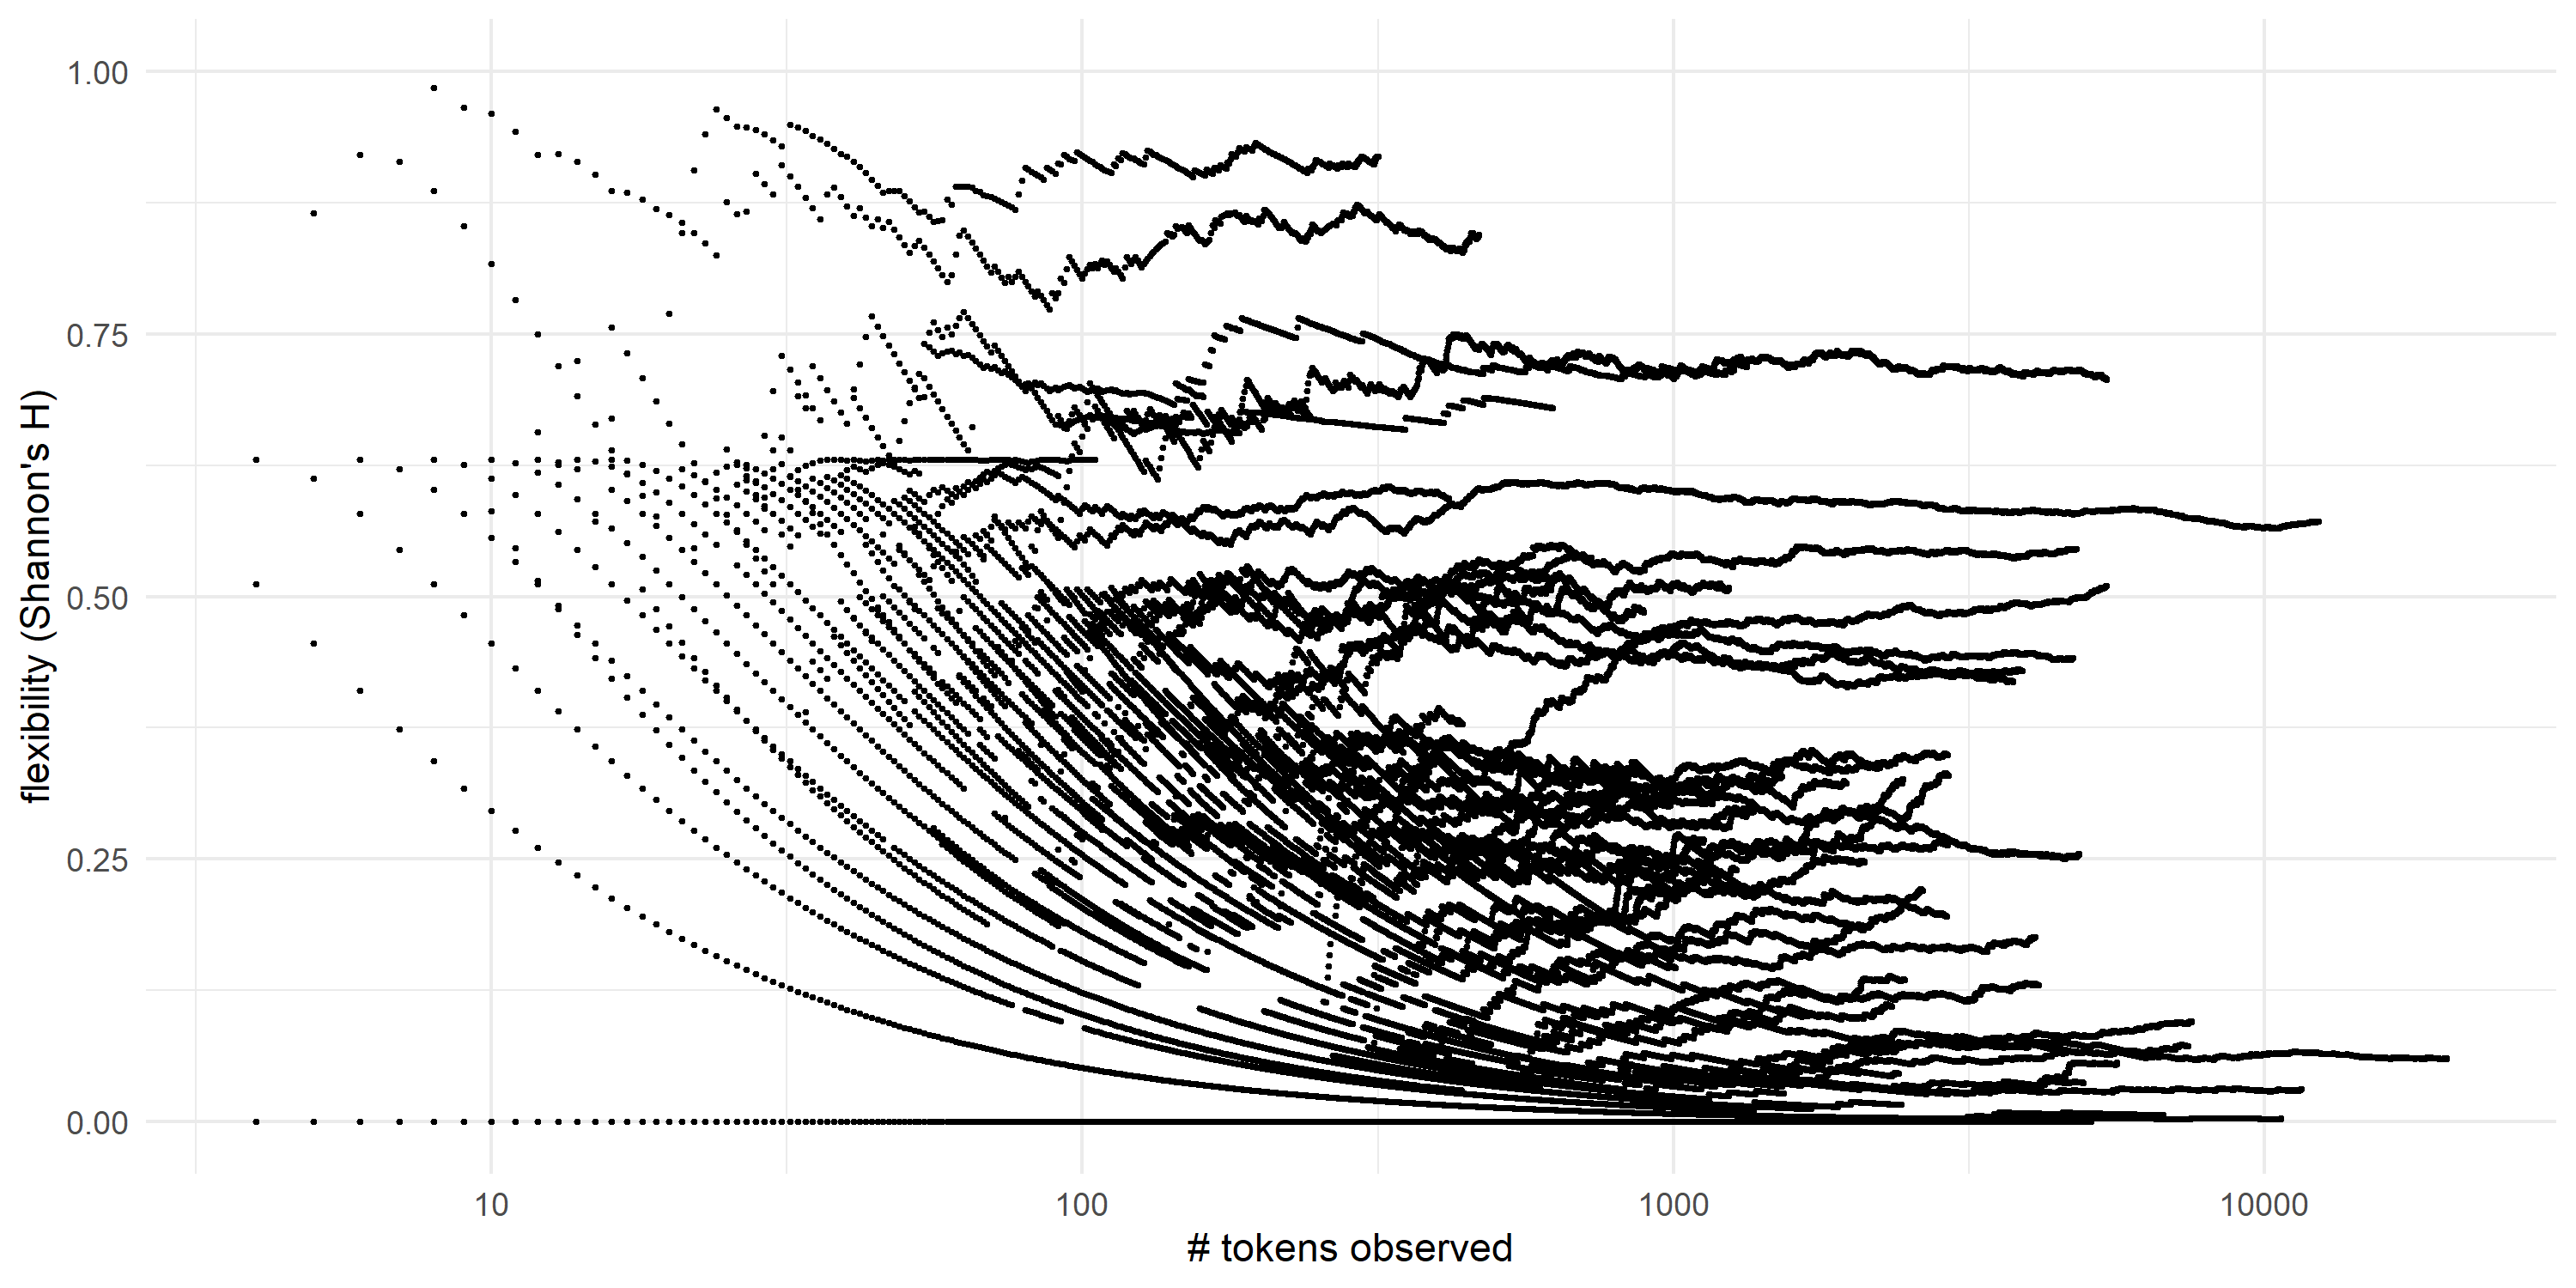
\includegraphics[width=\linewidth]{cumulative-flexibility-English-log.png}
\end{figure}

The first thing to notice from both plots of high-frequency words is that it takes a certain number of tokens for the flexibility of a word to become evident and stable. For \idx{English}, the trend lines are generally no longer stochastic after $\sim$1,000 tokens encountered (this can be more easily seen in \figref{fig:cumulative-flexibility-English-log}). If we take 1,000 tokens as a reliability threshhold for determining the flexibility of a lexical item, then no \idx{Nuuchahnulth} item appears with sufficient frequency in the corpus to be certain of its flexibility. That said, the flexibility of the ten words in the Nuuchahnulth sample appears to be relatively stable after 50–75 tokens. There are some words in the English sample which achieve a relatively stable flexibility rating as early as 100 tokens as well. One way to interpret these data is that, since some stems appear in a wider range of discourse contexts than others, it takes a higher number of tokens before the overall flexibility of those stems becomes evident; in contrast, the flexibility of stems that appear in a relatively small range of discourse contexts should become clear right away.

The second observation to make regarding these data is that, once the trend line for cumulative flexibility becomes smooth, it stays flat. This shows that corpora do not become more flexible as they increase in size. If this were true, we would expect to see a continual and gradual increase in flexibility for many of the stems in the dataset, and this is not the case.

On the other hand, by the time one encounters 5,000 tokens of a word in \idx{English}, there are no stems with a flexibility of zero. English flexibility ratings cluster in the lower range ($\sim0.3$), but when sufficient tokens are encountered, there do not seem to be any truly inflexible words. Therefore it does seem to be true (for English at least) that words will eventually display \emph{some} flexibility as the size of the corpus increases, but not that the overall flexibility of the word will increase.

We can also look at the data for each language in aggregate. \figref{fig:cumulative-mean-flexibility-English} shows the cumulative mean flexibility for \idx{English} per token encountered. Each time a new token of a lexical item was encountered, I calculated the current flexibility ratings of each lexical item encountered up to that point, and calculated their average. The resulting plot shows number of tokens encountered on the x-axis and mean flexibility for the entire corpus up to that point on the y-axis. \figref{fig:cumulative-mean-flexibility-Nuuchahnulth} shows parallel data for \idx{Nuuchahnulth}. Both graphs clearly show that the average flexibility of the corpus does not increase as the corpus grows larger. Instead it remains flat after a sufficient number of tokens are encountered.

\begin{figure}[h!]
  \centering
  \caption{Cumulative mean flexibility for \idx{English}}
  \label{fig:cumulative-mean-flexibility-English}
  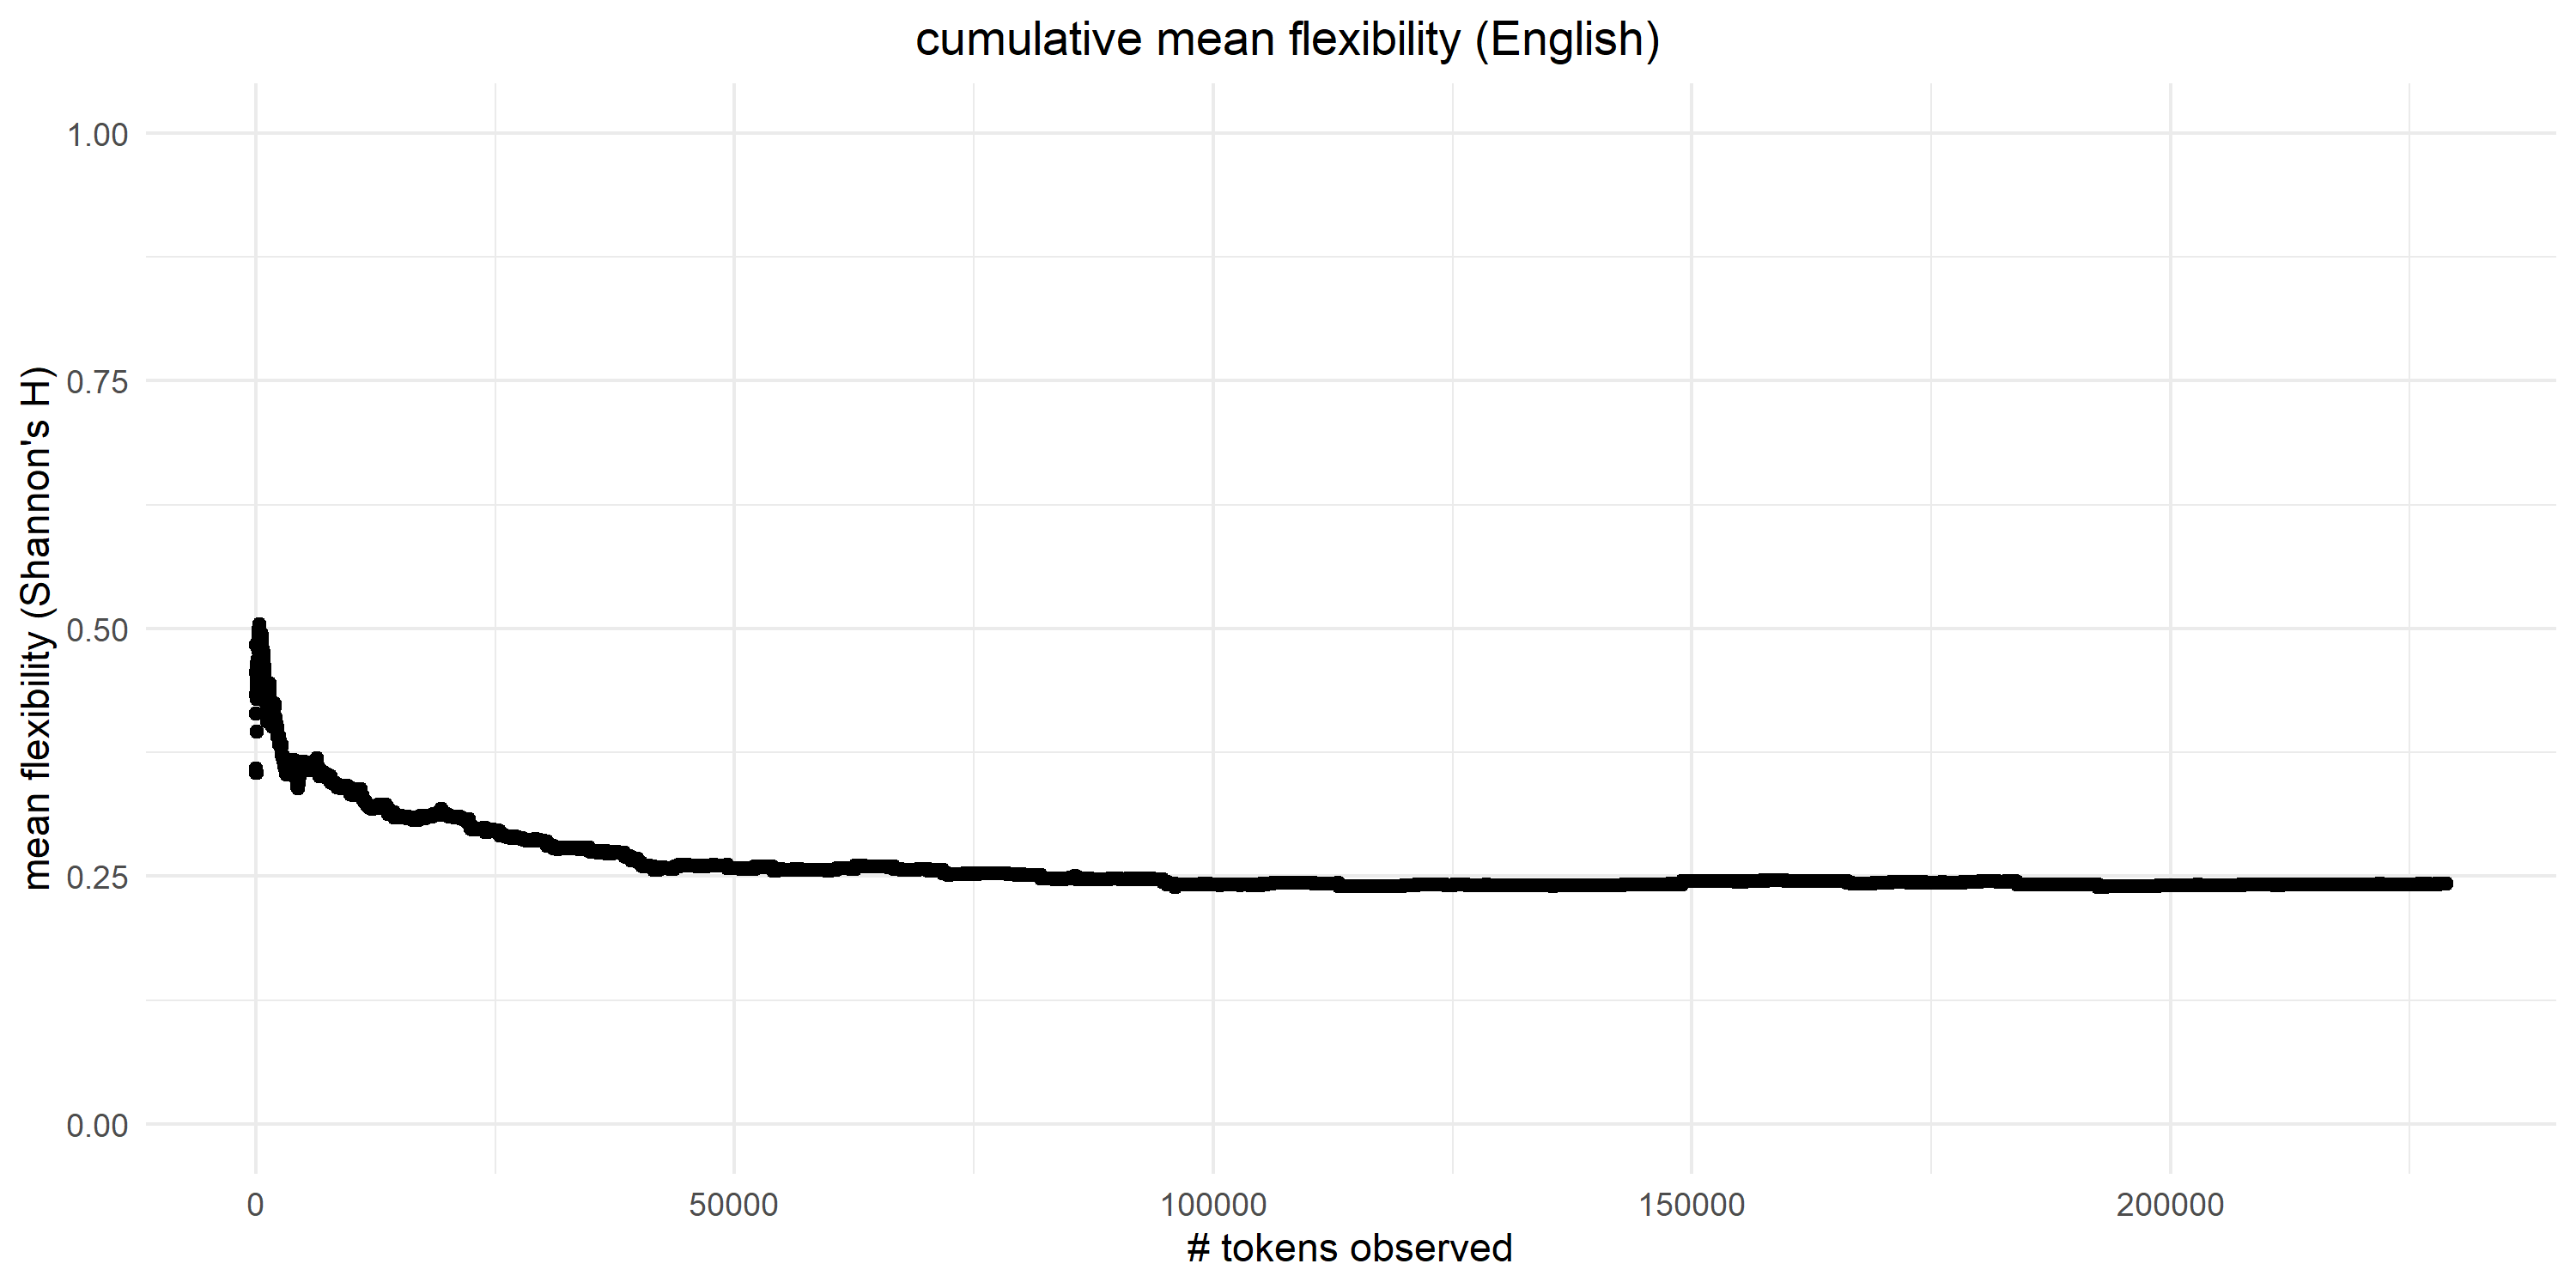
\includegraphics[width=\linewidth]{cumulative-mean-flexibility-English.png}
\end{figure}

\begin{figure}[h!]
  \centering
  \caption{Cumulative mean flexibility for \idx{Nuuchahnulth}}
  \label{fig:cumulative-mean-flexibility-Nuuchahnulth}
  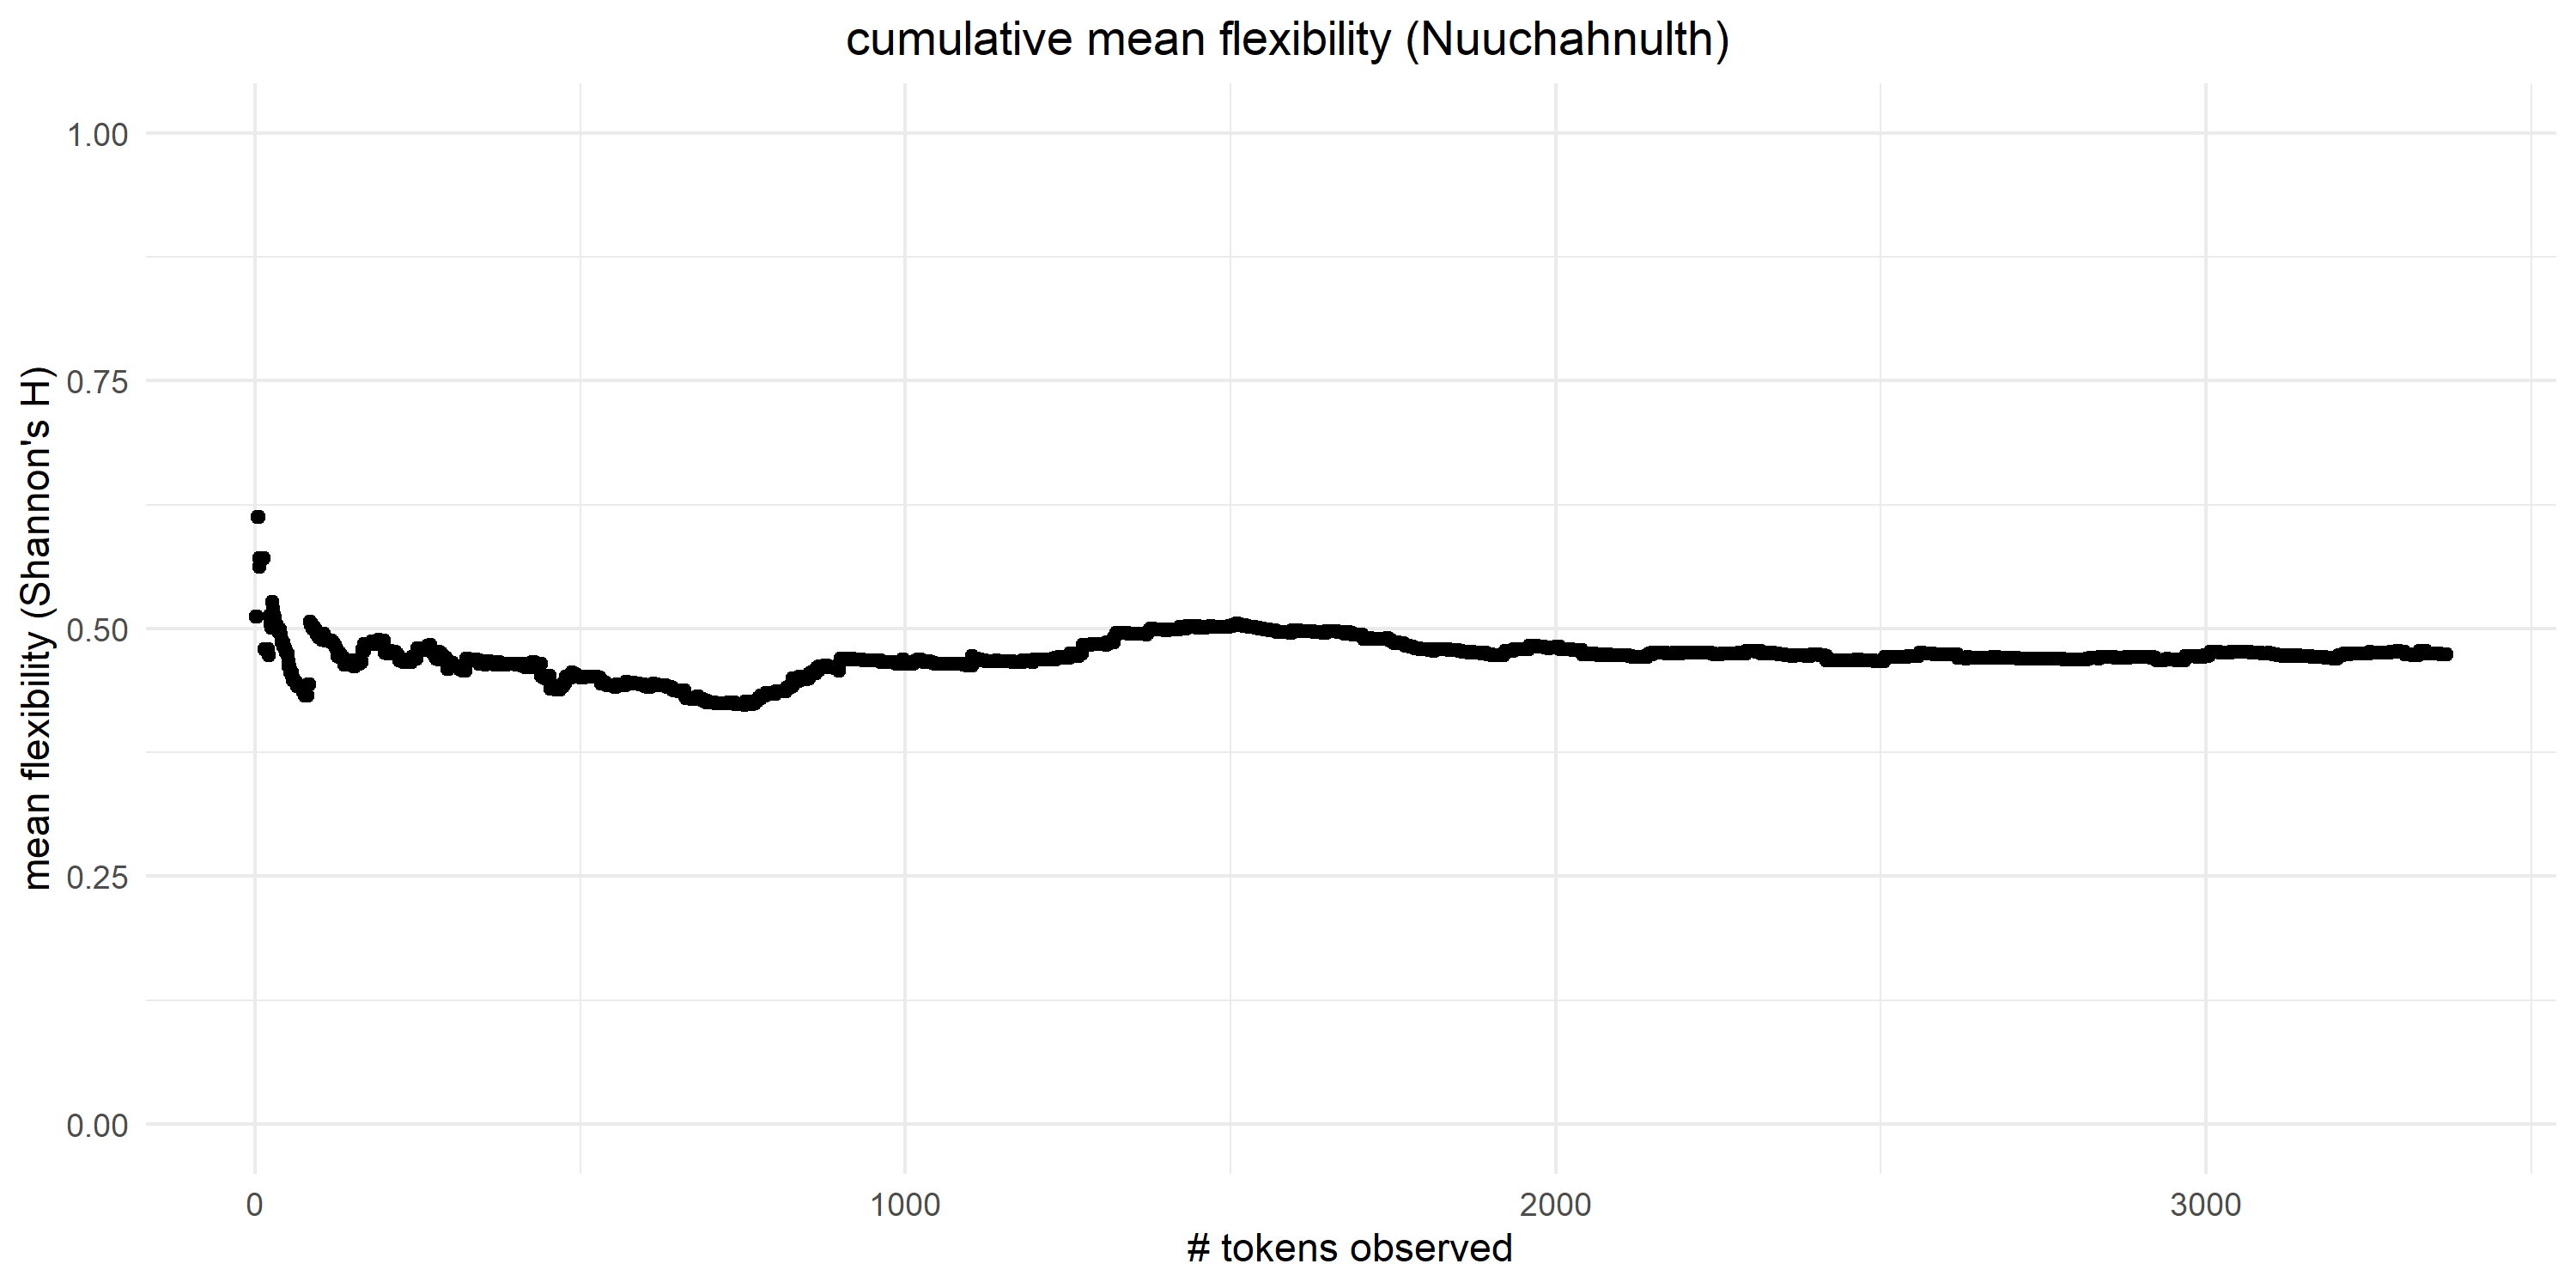
\includegraphics[width=\linewidth]{cumulative-mean-flexibility-Nuuchahnulth.png}
\end{figure}

To summarize, once enough tokens of a word are encountered to give a reliable flexibility rating, that flexibility rating does not increase as the number of tokens encountered continues to grow. Lexical items appear to have (synchronically) fixed degrees of flexibility, that vary from word to word. This suggests that the discourse functions of any given stem are conventionalized, so that speakers know which uses a word has, and generally use them with the same proportionate frequency. Logically, aggregating the data at the language level produces the same result: languages have (synchronically) fixed degrees of flexibility, that vary from language to language.

\section{R3: Lexical flexibility and frequency / dispersion}
\label{sec:4.5}

In this section I examine the interactions between lexical flexibility, token frequency, and corpus dispersion for individual lexical items. Given that many linguistic phenomena correlate with frequency / corpus dispersion, it is reasonable to investigate whether lexical flexibility displays such correlations as well. Are high frequency or evenly dispersed words more flexible than low frequency or unevenly dispersed words? This is an interesting question in part because if such a correlation were found the direction of causation could go in either direction. It may be that stems are more frequent precisely because they are more flexible—there is a wider range of discourse contexts that they can occur in. On the other hand, it could be that high frequency words are more cognitively accessible and therefore more prone to novel uses in discourse. Or, in contrast, a higher frequency could also result in a greater degree of entrenchment, so that high frequency words are less likely to be flexible.

To investigate the possible interactions among flexibility, frequency, and dispersion I deploy a Generalized Additive Model (GAM) in order to account for the possibility of interactions not just between flexibility and frequency / dispersion, but for interactions between frequency and dispersion as well. For example, it may be the case that there are correlations between flexibility and dispersion, but only for high frequency words. A Generalized Additive Model allows for the exploration of multiple interactions in this way.

Frequency is represented in this model as $\log_2$ of the relative frequency of the stem. Since relative frequency and corpus dispersion utilize different scales, I also use a tensor smooth to examine the combined contribution of frequency and dispersion to flexibility, over and above their individual contributions. I again used the 100-item sample for the English model, and the entire corpus for Nuuchahnulth.

\figref{fig:interaction-heat} shows heat maps of the interactions of the three variables for English and Nuuchahnulth. The x-axis shows $log_2$ of relative frequency, and the y-axis shows corpus dispersion as Deviation of Propotions ($DP$), with more evenly dispersed items to the bottom of the scale and less evenly dispersed items to the top of the scale. Light-colored areas indicate a high degree of flexibility, while dark-colored areas indicate a low degree of flexibility.

\begin{figure}
  \centering
  \caption{Interactions among frequency, dispersion, and flexibility for \idx{English} vs. \idx{Nuuchahnulth} (heat map)}
  \label{fig:interaction-heat}
  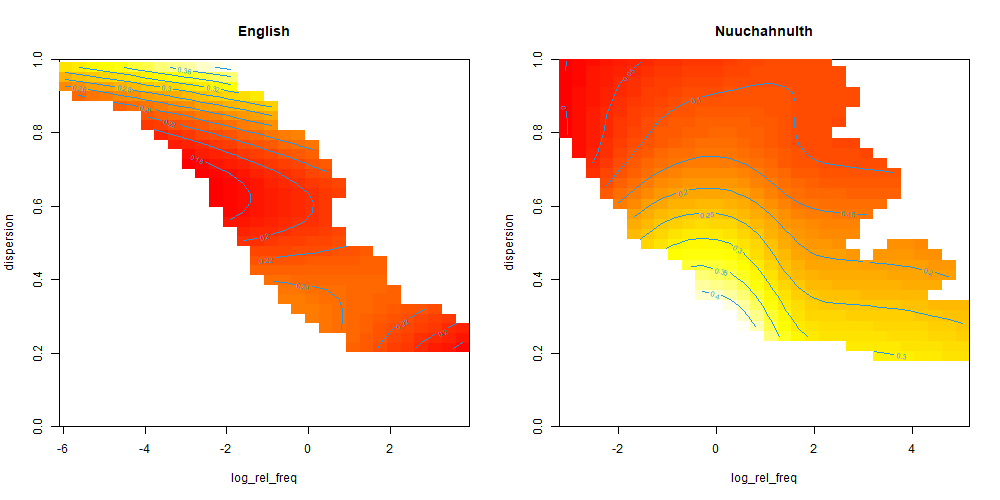
\includegraphics[width=\linewidth]{interaction-heat.png}
\end{figure}

\figref{fig:interaction-3D} shows 3D representations of the same data, rotated for ease of visualization. $\log_2$ relative frequency is shown on the x-axis (with higher relative frequency to the left—the reverse of \figref{fig:interaction-heat}), flexibility is shown on the y-axis (with higher flexibility at the top of the scale), and corpus dispersion is shown on the z-axis (with more evenly dispersed values further away).

\begin{figure}
  \centering
  \caption{Interactions among frequency, dispersion, and flexibility for \idx{English} vs. \idx{Nuuchahnulth} (3D map)}
  \label{fig:interaction-3D}
  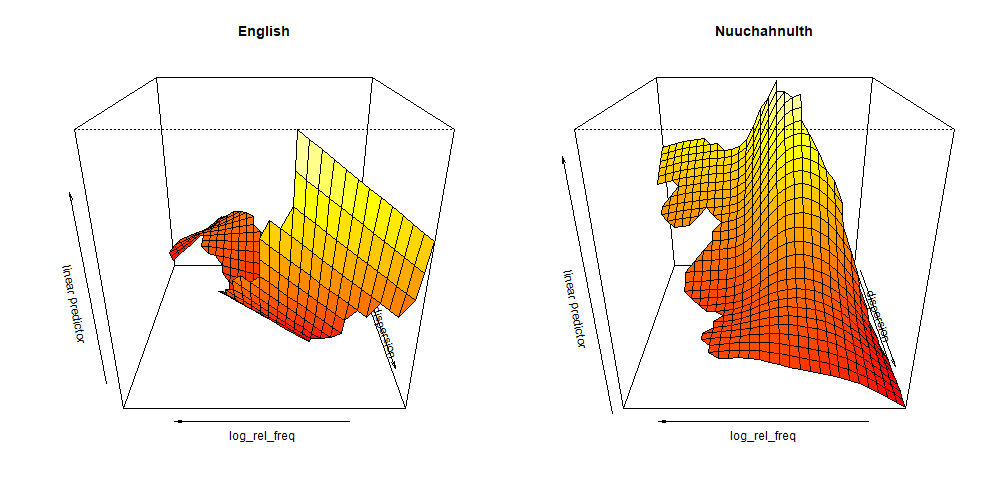
\includegraphics[width=\linewidth]{interaction-3D.png}
\end{figure}

In \idx{English}, high frequency, evenly dispersed items appear to have low flexibility ratings, while low frequency, unevenly dispersed items appear to have high flexibility ratings. However, none of the interactions for the English model are significant. The reason for this becomes apparent when we look at the same 3D interaction plot but with maps added at a standard deviation of 2, as in \figref{fig:interaction-3D-SD}. There is so much variability in the data for English that no firm conclusions can be drawn.

\begin{figure}
  \centering
  \caption{Interactions among frequency, dispersion, and flexibility for \idx{English} vs. \idx{Nuuchahnulth}, with standard deviations (3D map)}
  \label{fig:interaction-3D-SD}
  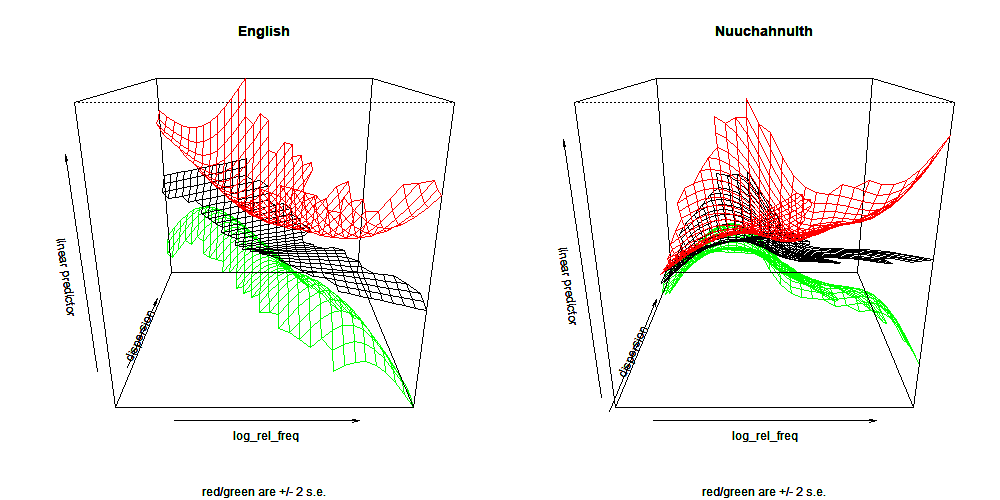
\includegraphics[width=\linewidth]{interaction-3D-SE.png}
\end{figure}

The model for \idx{Nuuchahnulth}, on the other hand, shows a couple of significant interactions. First, higher-frequency words show a greater degree of flexibility than lower-frequency words. This correlation is highly significant ($F = 37.582$, $p < .001$). Corpus dispersion, however, shows only a marginally significant correlation with flexibility ($F = 2.384$, $p < .1$), so no conclusion can be drawn regarding the direct relationship between corpus dispersion and flexibility. However, the combined interaction of corpus dispersion and relative frequency does correlate with flexibility, above and beyond the contribution provided by relative frequency alone ($F = 2.979$, $p < .05$). In total, these factors account for 18.2\% of the deviance in the data. Low frequency, unevenly dispersed items have low flexibility ratings, while high frequency, evenly dispersed items have higher flexibility ratings.

These results for \idx{Nuuchahnulth} should not be accepted unquestioningly as representative of the overall state of affairs for the language, however. Remember from \secref{sec:4.4} that a certain minimum threshhold of number of tokens is required in order to be certain of that word's flexibility. Given the relatively low frequencies of items in the Nuuchahnulth corpus, the flexibility ratings of many stems are likely inaccurate. In particular, the high incidence of items with zero-flexibility ratings is almost undoubtedly due to the small number of tokens encountered for those items. In fact, the 3D interaction plot for Nuuchahnulth in \figref{fig:interaction-3D-SD} shows that as stems increase in frequency, the standard deviation for their flexibility ratings grows dramatically, resembling that of English. Therefore it is likely that the strong correlations that currently appear for the Nuuchahnulth data would disappear with a larger corpus.

In summary, the data on lexical flexibility and frequency / corpus dispersion are not clear enough to draw any firm conclusions regarding their interactions.

\section{R4: The semantics of lexical flexibility}
\label{sec:4.6}

In this section I take a brief look at the semantics of lexical flexibility, in particular whether there are semantic commonalities to high or low flexibility words. I restrict myself here to aspects of the semantics of lexical items which can be discerned from the existing data and annotations used to answer other research questions for this project. Little additional data coding or annotation was done for the specific purpose of answering this research question. This section is therefore primarily exploratory, with the aim of discovering just what conclusions can be drawn about the semantics of lexical flexibility using merely the simple annotations of discourse functions prepared for this study. I begin with English before moving on to Nuuchahnulth.

\subsection{English}
\label{sec:4.6.1}

The first observation about the semantics of lexical flexibility in \idx{English} is purely anecdotal but nonetheless merits comment: the second most flexible word in the 100-item sample of English is \txn{back}, used 272 times for reference, 54 times for predication, and 143 times for modification, with a flexibility rating of $.844$. Going into this study, I postulated that body part terms would display a high degree of flexibility. The motivation for this hypothesis is that body part terms commonly undergo metaphorical extension into other domains, and in general make themselves available for all sorts of extensions of meaning. This is undoubtedly due to the fact that our experience of the world is necessarily mediated through our own bodies \parencite{LakoffJohnson1980}. The methods I chose to adopt in dissertation prevented any detailed exploration of this hypothesis, but it is notable that the only body part term in either of the 100-item samples is one of the single most flexible items in this study, anecdotally supporting the hypothesis that body part terms are in general highly flexible.

Several semantic classes stand out as being among the lowest flexibility words in the 100-item \idx{English} sample: indefinites; adult human animates (less so for non-adult humans, as the data for \txn{child} shows); property words denoting size, age, or physical properties; and words of cognition and perception generally have flexibility ratings lower than $0.100$, and most are within the 25 lowest flexibility words in the sample (exceptions are \txn{feel}, \txn{need}, and \txn{wonder}). Indefinites in particular rank lowest among the ratings (all with a flexibility rating of $0$). \tabref{tab:English-low-flexibility} shows the statistical data from the sample for each of the semantic classes just discussed, and their rank in terms of flexibility (out of the 100 items sampled). (Note that there are some ties for rank.)

\begin{table}
  \centering
  \caption{Low-flexibility stems in \idx{English}}
  \label{tab:English-low-flexibility}
  \begin{tabular}{ l r r r r r r r }
    \toprule
    Stem & Rel. Freq. & Disp. & Flex. & Ref. & Pred. & Mod. & Rank\\

    \midrule
    \multicolumn{6}{l}{Cognition \& Perception}\\
    \midrule
    need       &  0.833 & 0.501 & 0.220 & 164 &  2,475 &  3 & 43\\
    wonder     &  0.206 & 0.793 & 0.194 &  26 &    589 &  4 & 46\\
    feel       &  0.832 & 0.529 & 0.135 &  73 &  2,382 &  5 & 51\\
    decide     &  0.242 & 0.752 & 0.097 &   3 &    652 & 10 & 57\\
    think      &  6.477 & 0.262 & 0.060 & 162 & 20,089 & 58 & 66\\
    consider   &  0.146 & 0.834 & 0.058 &   0 &    336 &  4 & 67\\
    see        &  2.540 & 0.343 & 0.056 &  46 &  5,563 & 11 & 68\\
    understand &  0.275 & 0.724 & 0.053 &   4 &    752 &  3 & 71\\
    want       &  1.552 & 0.374 & 0.037 &   7 &  4,899 & 23 & 75\\
    know       & 13.729 & 0.214 & 0.030 &   7 & 11,496 & 51 & 76\\
    hate       &  0.140 & 0.840 & 0.026 &   0 &    442 &  2 & 78\\
    believe    &  0.312 & 0.709 & 0.014 &   0 &    953 &  2 & 81\\
    enjoy      &  0.481 & 0.677 & 0.005 &   0 &  1,485 &  1 & 90\\
    like       &  1.158 & 0.447 & 0.003 &   1 &  3,105 &  0 & 94\\

    \midrule
    \multicolumn{6}{l}{Human Animates}\\
    \midrule
    child   & 0.784 & 0.677 & 0.326 & 2,165 & 0 & 283 & 28\\
    woman   & 0.342 & 0.827 & 0.146 &   969 & 0 &  38 & 50\\
    man     & 0.287 & 0.765 & 0.101 &   752 & 1 &  16 & 56\\
    father  & 0.137 & 0.867 & 0.040 &   401 & 0 &   3 & 74\\
    person  & 0.360 & 0.690 & 0.013 & 1,011 & 1 &   1 & 84\\
    friend  & 0.390 & 0.653 & 0.012 & 1,237 & 1 &   1 & 85\\
    husband & 0.424 & 0.668 & 0.011 & 1,281 & 0 &   2 & 86\\

    \midrule
    \multicolumn{6}{l}{Indefinites}\\
    \midrule
    anything   & 0.755 & 0.449 & 0.000 & 2081  & 0 & 0 & 94\\
    everything & 0.606 & 0.518 & 0.000 & 1960  & 0 & 0 & 94\\
    something  & 1.665 & 0.341 & 0.000 & 5092  & 0 & 0 & 94\\
    thing      & 3.277 & 0.267 & 0.000 & 10649 & 0 & 0 & 94\\

    \midrule
    \multicolumn{6}{l}{Property Words}\\
    \midrule
    little & 1.738 & 0.362 & 0.511 & 1,345 & 0 & 4,062 & 15\\
    pretty & 1.170 & 0.440 & 0.170 &     1 & 1 &    51 & 49\\
    old    & 0.607 & 0.565 & 0.054 &     5 & 3 &   838 & 70\\
    big    & 0.830 & 0.474 & 0.046 &    21 & 0 & 2,381 & 72\\
    large  & 0.156 & 0.845 & 0.042 &     2 & 1 &   428 & 73\\
    hard   & 0.486 & 0.587 & 0.000 &     0 & 0 &   380 & 94\\

    \bottomrule
  \end{tabular}
\end{table}

It is easy to see why some of these classes of words would have such low flexibility ratings: each is highly prototypical of one particular discourse function. Adult human animates are one of the most prototypical classes of nouns crosslinguistically, while \txn{thing} and its variants are the most generic terms there are for referents. Words denoting size, age, or physical properties are among the core semantic classes for modifiers crosslinguistically \parencite{Dixon1977}. It is entirely unsurprising that these categories of words would nearly always be construed by speakers in the discourse functions that they are the most prototypical exemplars of. At the same time, these data show that such classification is not absolute. Even words that are strongly prototypical of a given discourse function are still occasionally used for other functions.\index{English}

It is less clear why words of cognition or perception have low flexibility ratings, except that in most cases there are corresponding overtly-derived referential terms which potentially block the use of the word as a referent: \txn{enjoy} is blocked by \txn{enjoyment}; \txn{believe} is blocked by \txn{belief}; \txn{hate} is blocked by \txn{hatred}; \txn{know} is blocked by \txn{knowledge}; and so on. These referential counterparts do not necessarily \emph{prevent} the use of these stems as referents (e.g. \textit{to be in the \textbf{know}}), but they are likely a significant contributing factor. In fact, the highest flexibility words in this category are ones which do not have morphologically-derived counterparts: \txn{feel}, \txn{need}, and \txn{wonder}. \textcite[111]{Farrell2001} reports finding the same pattern for English: unless a word is \enquote{pre-empted or blocked}, it generally exhibits flexible behavior.


Regardless, it is unclear why these words have morphologically derived referential counterparts but most of the highest-flexibility words such as \txn{paint}, \txn{work}, \txn{order}, and \txn{transfer} do not.\index{English}

\subsection{Nuuchahnulth}
\label{sec:4.6.2}

When we look at the semantic classes that align with high and low flexibility in \idx{Nuuchahnulth}, one class in particular stands out as being especially flexible: property-denoting words, and especially numerals and quantifiers. 12 of the top 20 most flexible stems in Nuuchahnulth are property words. With few exceptions, property-denoting words in Nuuchahnulth have high flexibility ratings, above $0.5$. All of the core deictic stems in Nuuchahnulth also feature in the top 25 most flexible words. The statistical data for both these classes of stems, along with their rank in terms of flexibility, are listed in \tabref{tab:Nuuchahnulth-high-flexibility}.

\begin{table}
  \centering
  \caption{High-flexibility stems in \idx{Nuuchahnulth}}
  \label{tab:Nuuchahnulth-high-flexibility}
  \begin{tabular}{ l l r r r r r r r }
    \toprule
    Stem & Gloss & Rel. Freq. & Disp. & Flex. & Ref. & Pred. & Mod. & Rank\\

    \midrule
    Property Words\\
    \midrule
    hiš      & all        & 0.956 & 0.580 & 0.985 &  3 &  3 & 2 &  1\\
    ʔaƛakʷaɬ & eight      & 0.956 & 0.614 & 0.921 &  2 &  3 & 1 &  2\\
    muː      & four       & 0.837 & 0.755 & 0.921 &  2 &  3 & 1 &  3\\
    čamiḥta  & proper(ly) & 0.717 & 0.566 & 0.921 &  2 &  3 & 1 &  4\\
    ʔuːš     & some       & 2.391 & 0.556 & 0.920 &  9 &  8 & 3 &  5\\
    c̓awaːk   & one        & 1.673 & 0.437 & 0.842 &  3 &  8 & 2 &  6\\
    ƛaʔuː    & another    & 2.271 & 0.322 & 0.835 & 11 &  6 & 2 &  7\\
    hiːtkin  & strange    & 0.717 & 0.773 & 0.790 &  1 &  4 & 1 &  8\\
    ʔaƛa     & two        & 1.434 & 0.423 & 0.783 &  1 &  7 & 3 &  9\\
    ʔiːḥ     & big        & 1.554 & 0.561 & 0.719 &  1 &  9 & 3 & 12\\
    ʔaya     & many       & 4.064 & 0.424 & 0.652 &  2 & 23 & 6 & 14\\
    mixt     & aged       & 0.478 & 0.886 & 0.631 &  2 &  2 & 0 & 21\\
    ʔiːč̓im   & old        & 0.598 & 0.801 & 0.613 &  2 &  3 & 0 & 29\\

    \midrule
    Deictic Words\\
    \midrule
    ḥaːɬ   & there      &  2.510 & 0.506 & 0.761 &  5 & 14 &  2 & 10\\
    ʔaḥ    & this       & 12.551 & 0.317 & 0.732 & 73 & 16 & 14 & 11\\
    ʔaḥʔaː & that       & 12.790 & 0.275 & 0.672 & 55 & 48 &  1 & 13\\
    ʔaḥku· & right.here &  0.717 & 0.688 & 0.631 &  3 &  3 &  0 & 20\\
    hiɬ    & there      &  6.216 & 0.393 & 0.606 & 20 & 32 &  0 & 30\\

    \bottomrule
  \end{tabular}
\end{table}

What accounts for the consistently high flexibility rating for property words? Why is it that property words are so rigid in English yet so flexibile in Nuuchahnulth? First, \idx{Nuuchahnulth} does not have any dedicated morphosyntactic constructions that express the function of modification, except that modifiers precede their head syntactically and take no inflectional affixes when they do so. Yet while this syntactic construction is available to speakers, its use is fairly uncommon. Instead, speakers avail themselves of two strategies for communicating property concepts: a) lexical affixation, and b) construing property concepts as either referents or predicates.

\idx{Wakashan} languages and the languages of the Pacific Northwest in general are well known for their use of \dfn{lexical affixes}, affixes with concrete lexical meanings rather than grammatical / functional ones \parencite{Mithun1997}. \idx{Nuuchahnulth}'s large set of lexical suffixes allows speakers to use property-denoting roots in complex stems, where the root denotes the property being attributed, and the lexical suffix denotes the referent being modified. Example \exref{ex:4.1} shows two such uses of property-denoting roots.

\begin{exe}
  \ex\label{ex:4.1}
  \exinfo{\idx{Nuuchahnulth} (Wakashan > Southern Wakashan)}
  \begin{xlist}

    \ex\label{ex:4.1a}
    \gllll niyasu           hihiqtup\\
           ni‑yasu·         \em{hihiq}‑tu·p\\
           dip‑in.water     \em{all}‑thing\\
           sink.under.water everything\\
           \tln{everything was under the water}
    \exsource[Flood 027]{Little2003}

    \ex\label{ex:4.1b}
    \gllll ʔaƛc̓iq\\
           \em{ʔaƛ}‑c̓iq\\
           \em{two}‑canoes\\
           two.canoes\\
           \tln{there were two boats}
    \exsource[GL 099]{Louie2003}

  \end{xlist}
\end{exe}

\noindent The use of property-denoting roots with lexical affixes is by far the most common strategy for attributing properties to referents in \idx{Nuuchahnulth}. The choice between a bare modifier and the use of lexical affixes is intimately connected with information flow in discourse. Already-activated discourse referents are typically expressed through lexical affixes, whereas newly-introduced discourse referents are presented as independent noun phrases \parencite[887--889]{Mithun1984}. \textcite[144]{Nakayama2001} also shows that referentiality is a key deciding factor between the two constructions.

The other manner by which speakers express property concepts is with either referring or predicating constructions. The fact that speakers use \emph{either} referring or predicating constructions (as opposed to just referring constructions or just predicating constructions) likely has to do with the dual function of property concepts identified by \textcite{Thompson1989}. In a corpus analysis of English and Mandarin, \citeauthor{Thompson1989} finds that property words have primarily two functions in discourse: to introduce new discourse-manipulable referents, and to predicate attributes of an already-known referent. In English these two functions are realized via attributive adjectives and predicative adjectives respectively. \idx{Nuuchahnulth} appears to follow a similar pattern: when a property word is used to introduce a new referent into the discourse, it typically appears as an independent word modifying a nominal head. As with the English data from \posscitet{Thompson1989} study, the head is typically a semantically empty or generic referent whose primary function is to serve as a carrier of the property word. Example \exref{ex:4.2} demonstrates this phenomenon in Nuuchahnulth.

\begin{exe}
  \ex\label{ex:4.2}
  \exinfo{\idx{Nuuchahnulth} (Wakashan > Southern Wakashan)}
  \begin{xlist}

    \ex\label{ex:4.2a}
    \gllll ʔatquu              \em{čamiḥta} quuʔas qawiqaaɬ\\
           ʔat‑quː             \em{čamiḥta} quːʔas qawiqaːɬ\\
           even.if‑\gl{cond.3} \em{proper}  person Qawiqaalth\\
           although            \em{proper}  person Qawiqaalth\\
           \tln{although Qawiqaalth was a proper person}
    \exsource[Qawiqaalth 011]{Louie2003}

    \ex\label{ex:4.2b}
    \gllll ʔucḥinƛ        ƛuɬaqakʔi                      ḥakʷaaƛ  muuḥinƛas\\
           ʔu‑cḥinƛ       \em{ƛuɬ}‑aq‑ak‑ʔi·               ḥaːkʷaːƛ muːḥinƛ‑as\\
           she‑marry.to   \em{nice}‑very‑\gl{dur}‑\gl{def} girl     sawbill‑female\\
           get.married.to very.beautiful                 girl     Sawbill.woman\\
           \tln{He got married to very beautiful Sawbill Woman}
    \exsource[Mink 287]{Louie2003}

  \end{xlist}
\end{exe}

\noindent By contrast, when a property is being predicated of an already-established discourse referent, the lexical affix strategy is used instead.

Returning to the discussion of semantic classes, if we focus on just the numerals, we find a potential trend: for the numerals 1–3, the flexibility of the stems decrease as their numeric values increase. The cardinal numbers and their flexibility ratings are shown in numeric order in \tabref{tab:Nuuchahnulth-numerals} for those stems that occur in the corpus. Given the low frequencies involved for these stems, it would be unwise to make strong claims about the potential trend in this table. The irregularity here is of course for the numerals \tln{four} and \tln{eight}. However, since all the instances of \tln{four} and \tln{eight} appear in the same text, the values for these stems may not be representative. As such, the data are potentially suggestive of the idea that cardinal numerals adhere to an implicational hierarchy, wherein the flexibility of a numeral decreases as its numeric value increases. If true, this trend would be in line with other well-documented implicational universals for cardinal numerals \parencites{DehaeneMehler1992}[141]{Croft2003}.\index{Nuuchahnulth}

\begin{table}[h!]
  \centering
  \caption{Flexibility of numerals in \idx{Nuuchahnulth}}
  \label{tab:Nuuchahnulth-numerals}
  \begin{tabular}{ l l r r r r r r }
    \toprule
    Stem & Gloss & Rel. Freq. & Disp. & Flex. & Ref. & Pred. & Mod.\\
    \midrule
    c̓awaːk   & one   & 1.673 & 0.437 & 0.842 & 3 & 8 & 2\\
    ʔaƛa     & two   & 1.434 & 0.423 & 0.783 & 1 & 7 & 3\\
    qacc̓a    & three & 0.598 & 0.694 & 0.512 & 0 & 3 & 1\\
    muː      & four  & 0.837 & 0.755 & 0.921 & 2 & 3 & 1\\
    ʔaƛakʷaɬ & eight & 0.956 & 0.614 & 0.921 & 2 & 3 & 1\\
    \bottomrule
  \end{tabular}
\end{table}

Much as in \idx{English}, animate human beings are generally among the lower-flexibility stems in \idx{Nuuchahnulth} (below $0.5$), although their ratings are still higher than those for English. The animate human stems and their flexibility ratings are shown in \tabref{tab:Nuuchahnulth-low-flexibility}. Of particular note is the fact that the word \txn{quːʔas} \tln{person, man} has one of the lowest flexibility ratings in the Nuuchahnulth corpus (excluding those with ratings of zero). Yet this was the very stem that \textcite{Swadesh1939b} used to demonstrate Nuuchahnulth's extreme flexibility! This is an excellent example of why we need more empirical coverage for the study of lexical flexibility—this claim about the flexibility of the word \tln{person, man} in Nuuchahnulth has been repeated verbatim for nearly a century, but entirely unbacked by the kind of comprehensive data needed to support it. The marginal flexibility of \tln{person, man} and other human animates does however illustrate that even highly prototypical referents exhibit degrees of flexibility.

\begin{table}
  \centering
  \caption{Low-flexibility stems in \idx{Nuuchahnulth}}
  \label{tab:Nuuchahnulth-low-flexibility}
  \begin{tabular}{ l l r r r r r r }
    \toprule
    Stem     & Gloss  & Rel. Freq. & Disp. & Flex. & Ref. & Pred. & Mod.\\
    \midrule
    ɬuːcma   & wife   & 2.988      & 0.559 & 0.477 & 18   & 5     & 0  \\
    ḥaw̓iɬ    & chief  & 4.184      & 0.549 & 0.417 & 26   & 6     & 0  \\
    ḥaːkʷa·ƛ & girl   & 2.869      & 0.868 & 0.158 & 23   & 1     & 0  \\
    quːʔas   & person & 9.682      & 0.341 & 0.106 & 78   & 2     & 0  \\
    \bottomrule
  \end{tabular}
\end{table}

Because the \idx{Nuuchahnulth} corpus is a fully glossed interlinear corpus, it is possible to answer certain questions that cannot be as easily answered for the English corpus. In particular, it is a fairly straightforward task to analyze relationships between specific kinds of morphemes and discourse function. Nuuchahnulth has a definite suffix \txn{-ʔi·}, for example, which is sometimes said to have a disambiguating function \parencites[60-63]{Mithun1999}[48]{Nakayama2001}. In most cases, context and the meaning of the stem serve to disambiguate referential versus predicative uses of the same stem. However, in cases where a stem is non-prototypically serving as a referent, the definite suffix is more likely to appear.

I set out to investigate the possible connection between the use of the definite marker and non-prototypical uses of stems by examining the frequency with which the definite marker occurs with stems marked for different aspects. \parentext{Note that in \idx{Nuuchahnulth}, aspect markers are not limited to just predicative stems. They may appear with referential uses of stems as well \parencite[47--48]{Nakayama2001}.} The intuition behind this procedure is that some Nuuchahnulth aspects, like the continuative or progressive aspects, are more prototypically predicative in their meaning than others, such as the durative or momentaneous aspects. Thus, I hypothesized that the definite marker would occur more frequently on continuative and progressive aspects than the durative or momentaneous aspects.

Unfortunately, there were insufficient data to answer this question. The reason the data are insufficient is telling, however. To begin with, the definite marker appears on 213 of the 1935 attested stems in the corpus (11.01\%). However, only 17 of those stems (7.98\%) also ever appear with an aspect marker (either continuative, durative, momentaneous, or telic). The dataset is simply too small to draw any conclusions about the interaction of definiteness and aspect. That said, the \emph{near} mutually exclusive distribution of aspect markers and the definite marker in \idx{Nuuchahnulth} is noteworthy precisely because it provides additional support for \posscitet{HopperThompson1984} claim that the prototypical uses of lexical items exhibit inflectional behaviors characteristic of their class. Even in a language with extensive flexibility like Nuuchahnulth, that flexibility is constrained by typological universals.
